\chapter{Разработка алгоритмов автоматического распознавания речевых команд на основе свёрточных нейронных сетей глубокого обучения} \label{chapt4}

В данном разделе приведено описание разработки алгоритмов автоматического распознавания речевых команд на основе свёрточных нейронных сетей глубокого обучения.
Теория по данному типу искусственных нейронных сетей описана в подразделе \ref{sect1_3_3}.
При проведении экспериментов на нейронных сетях использовались параметрические портреты меньших размеров, чем при тестировании ранее предложенными алгоритмами.
Лучшие результаты при распознавании слов были получены на портретах с 18 частотными полосами и 25 временными интервалами.
При распознавании фраз в использованных параметрических портретах также было 18 частотных полос, а число временных интервалов увеличено с 25 до 75, так как фразы в среднем состоят приблизительно из трёх слов.
В данном случае для уменьшения размерности параметрических портретов может быть использован алгоритм сжатия портретов на основе полиномов Чебышёва, описанный в подразделе \ref{sect2_4}.
Также для всех портретов из обучающей выборки может быть применено разбиение на однородные части и выравнивание найденных частей относительно друг друга для каждого слова.
Подробное описание алгоритма разбиения параметрического портрета слова на однородные части приведено в подразделе \ref{sect2_2}.

Для обучения всех нейронных сетей прямого распространения принято использовать метод обратного распространения ошибки.
Существуют пакетная, стохастическая и смешанная, мини-пакетная реализации данного метода.
Последняя реализация самая используемая на текущий момент и будет применяться в этом разделе.
К её особенностям относится некоторая случайность в процессе обучения, что приводит к немного различающимся результатам распознаваний при одинаковых параметрах обучения.
Более того, в некоторых нейронных сетях применяется регуляризация, которая также вносит небольшую случайность в процесс обучения.
Отсюда можно сделать вывод, что все результаты являются примерными и могут не воспроизводиться точь-в-точь при повторных запусках.

Моделирование искусственных нейронных сетей проводилось в программном комплексе, написанном на языке программирования Python с использованием библиотек TensorFlow и TFLearn.
TensorFlow --- это низкоуровневая библиотека с открытым исходным кодом, разработанная для решения задач построения и обучения нейронных сетей \cite{tensorflow}.
TFLearn --- высокоуровневая библиотека для упрощения работы с нейронными сетями, является оболочкой для библиотеки TensorFlow \cite{tflearn}.
Обе библиотеки могут производить вычисления как на центральном процессоре, так и на графическом процессоре.
Использование последнего является приоритетным, так как такие процессоры содержат очень много малопроизводительных ядер, что хорошо подходит для процесса обучения нейронных сетей, алгоритм которого поддаётся эффективному распараллеливанию.
Для эффективного использования графического процессора в работе программы применяется программно-аппаратная архитектура параллельных вычислений CUDA, активно использующая приведённые выше подключаемые библиотеки \cite{cuda}.

%\newpage
%============================================================================================================================

\section{Оценки работоспособности традиционных сетей типа одно- и двухслойных персептронов в задаче распознавания речевых команд} \label{sect4_1}

Первоначально в нейронных сетях были проведены оценки работоспособности традиционных сетей типа одно- и двухслойных персептронов в задаче распознавания речевых команд.
Прежде всего, исходя из стандартных рекомендаций выбиралась структура нейронной сети.
Для персептронов это количество нейронов в каждом слое.
После этого подбирались параметры сети, такие как скорость обучения, количество итераций, размер пачки и коэффициент регуляризации.
Далее, для выбранных оптимальных параметров проводилось распознавание всех записей на обучающей базе, состоящей из одного и двух дикторов.

Однослойный персептрон состоит из входного слоя, содержащего $18 \times 25 = 450$ входов (равно размеру входящего параметрического портрета) и выходного слоя, состоящего из 20 нейронов (равно количеству распознаваемых слов).
Сеть является полносвязной, то есть каждый входной элемент соединён синапсами с выходными нейронами.
Получается, что в нейронной сети есть $450 \times 20 = 9000$ синапсов или весов, которые подбираются в процессе обучения.
Для последнего слоя используется функция softmax для нормировки полученных выходных вероятностей.
Для обучения однослойного персептрона в качестве функции потерь используется перекрёстная энтропия.
В персептроне с одним слоем регуляризация обычно не применяется.
В процессе обучения используется вариант оптимизации Adam (adaptive moment estimation --- адаптивная оценка моментов) для стохастического градиентного спуска.
На рисунке \ref{fig:perceptron1_my} представлена структура полученного однослойного персептрона.

\begin{figure}[h]
	\centering
	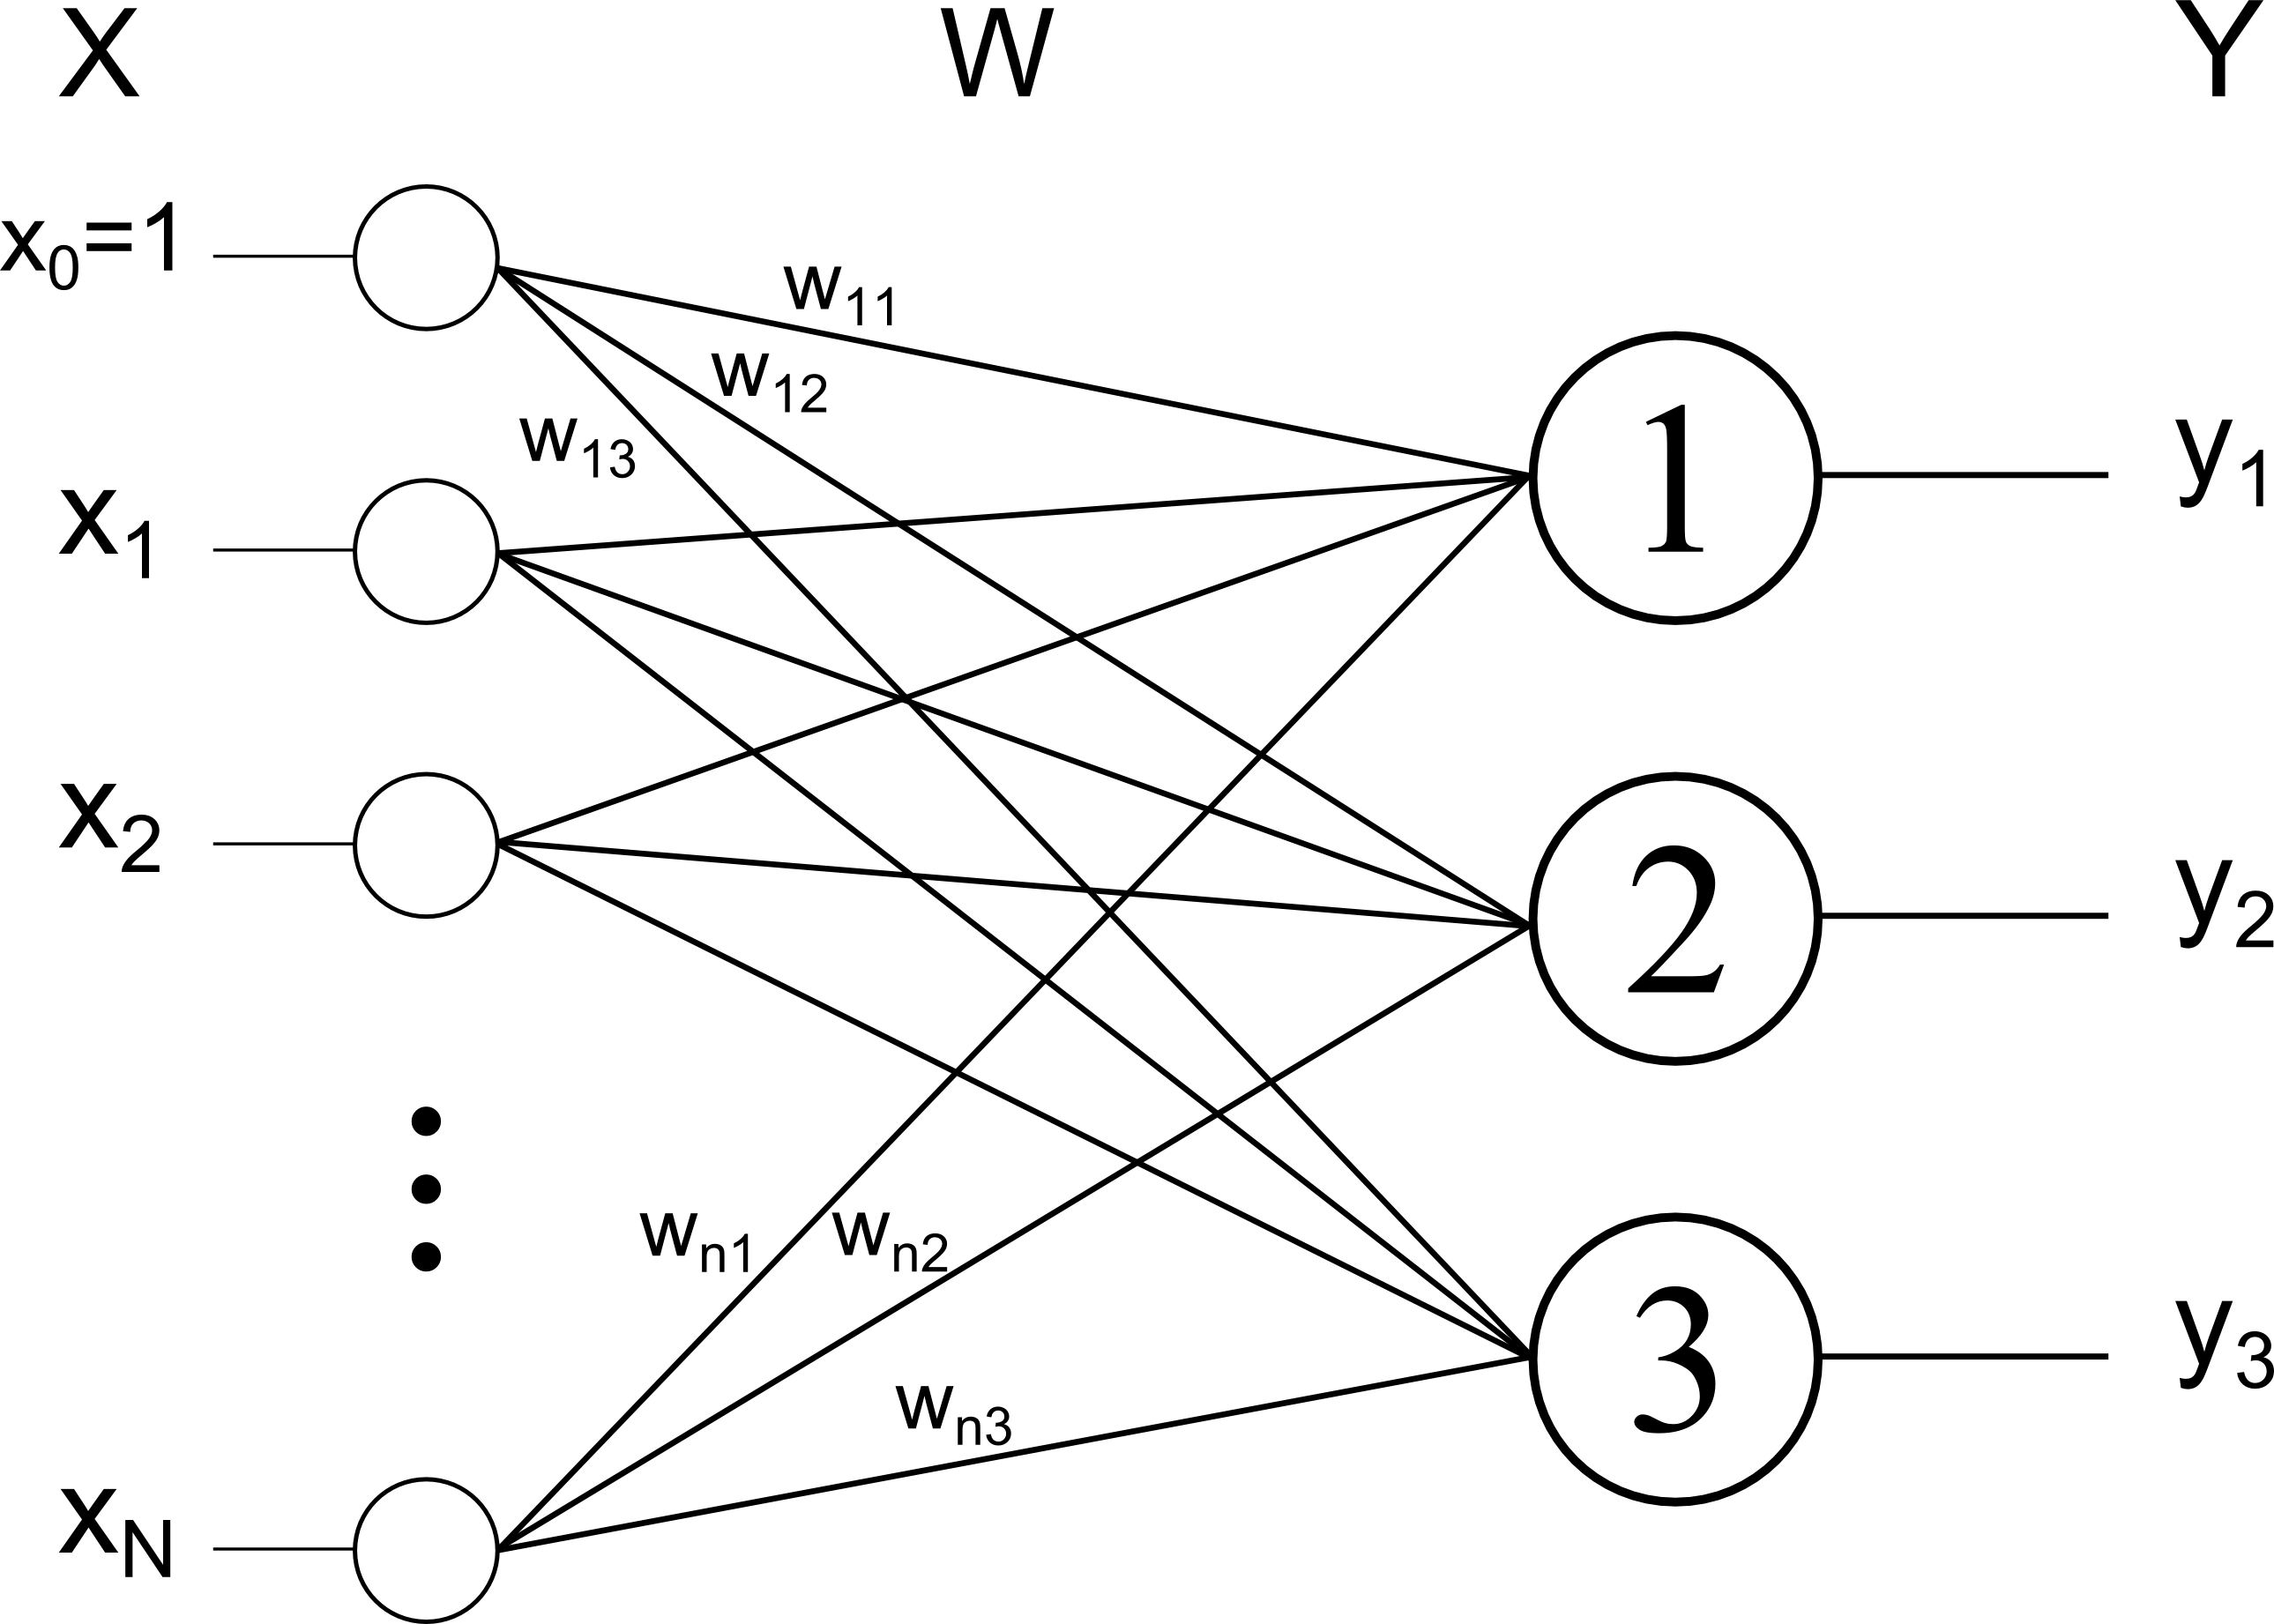
\includegraphics[width=12cm]{perceptron1_my.png}
	\caption{Структура используемого однослойного персептрона}
	\label{fig:perceptron1_my}
\end{figure}

Для однослойного персептрона сначала подбиралось количество итераций обучения и скорость обучения при фиксированном размере пачки, равному 600 записей.
Результаты подбора приведены в таблице \ref{tab:mlp1_bf_iter_pace}, оптимальное значение выделено жирным.

\begin{table}[h]
	\centering
	\caption{Подбор количества итераций и скорости обучения для однослойного персептрона, в таблице указан процент неправильных распознаваний}
	\label{tab:mlp1_bf_iter_pace}
	\begin{tabular}{| l | c | c | c | c | c | c | c | c | c |}
		\hline
		Скорость & \multicolumn{5}{c|}{Количество итераций} \\
		\hhline{~---------}
		обучения \phantom{00} & \phantom{000} 100 \phantom{000} & \phantom{000}1000\phantom{000} & \phantom{000}3000\phantom{000} & \phantom{00} 10000 \phantom{00} & \phantom{00} 30000 \phantom{00} \\
		\hline
		0.00001  & 95.68 & 93.80 & 94.36 & 91.02 & 53.87 \\
		0.00003  & 95.31 & 94.12 & 92.48 & 66.04 & 40.00 \\
		0.0001	 & 95.49 & 90.79 & 71.89 & 43.99 & 34.81 \\
		0.0003	 & 95.93 & 74.85 & 49.05 & 39.88 & 33.16 \\
		0.001  	 & 91.96 & 51.37 & 43.33 & 38.07 & 31.64 \\
		0.003 	 & 82.46 & 44.51 & 41.49 & 38.93 & 33.57 \\
		0.01 	 & 54.64 & 40.15 & 39.47 & 36.25 & 37.93 \\
		0.03 	 & 40.85 & 37.48 & 34.53 & 31.14 & 31.56 \\
		0.1 	 & 23.96 & 24.25 & \textbf{23.56} & 22.45 & 22.59 \\
		0.3 	 & 19.65 & 19.28 & 20.33 & 18.13 & 19.24 \\
		1 		 & 18.40 & 19.34 & 20.32 & 19.70 & 18.24 \\
		\hline
	\end{tabular}
\end{table}
Оптимальное количество итераций получилось равным 3000, а оптимальная скорость обучения --- 0.1.

Затем подбиралось количество итераций обучения и размер пачки при фиксированной скорости обучения, равной 0.1.
Результаты подбора приведены в таблице \ref{tab:mlp1_bf_iter_batch}, оптимальное значение выделено жирным.

\begin{table}[h]
	\centering
	\caption{Подбор количества итераций и размера пачки для однослойного персептрона, в таблице указан процент неправильных распознаваний}
	\label{tab:mlp1_bf_iter_batch}
	\begin{tabular}{| l | c | c | c | c | c | c | c | c | c |}
		\hline
		Размер	 & \multicolumn{5}{c|}{Количество итераций} \\
		\hhline{~---------}
		пачки \phantom{0000} & \phantom{000} 100 \phantom{000} & \phantom{000}1000\phantom{000} & \phantom{000}3000\phantom{000} & \phantom{00} 10000 \phantom{00} & \phantom{00} 30000 \phantom{00} \\
		\hline
		10		 & 79.16 & 79.38 & 79.92 & 79.35 & 79.12 \\
		30 		 & 61.11 & 61.85 & 61.64 & 57.45 & 58.35 \\
		60 		 & 48.60 & 44.98 & 48.23 & 46.13 & 46.12 \\
		120 	 & 36.97 & 34.37 & 37.01 & 34.99 & 34.93 \\
		200 	 & 30.00 & 31.75 & 30.22 & 26.52 & 28.96 \\
		300 	 & 27.70 & 24.25 & 27.15 & 25.85 & 28.56 \\
		450 	 & 25.34 & 25.13 & 24.23 & 22.78 & 26.93 \\
		600 	 & 24.54 & 22.16 & \textbf{23.28} & 22.81 & 25.65 \\
		\hline
	\end{tabular}
\end{table}

Оптимальное количество итераций получилось равным 3000, а оптимальный размер пачки --- 600.

Оптимальными параметрами нейронной сети стали: количество итераций обучения --- 3000, скорость обучения --- 0.1 и размер пачки 600.
Результаты распознаваний для однослойного персептрона приведены в таблице \ref{tab:mlp1_dictor1} для случая обучения на наборе данных, состоящем из записей одного диктора, и в таблице \ref{tab:mlp1_dictor2} для случая обучения на наборе данных, состоящем из записей двух дикторов.

\begin{table}[h]
	\centering
	\caption{Результаты распознавания слов однослойным персептроном на обучающем наборе из одного диктора, в таблице указан процент неправильных распознаваний}
	\label{tab:mlp1_dictor1}
	\begin{tabular}{| l | c | c | c | c | c | c | c | c | c |}
		\hline
		Набор & \multicolumn{9}{c|}{Диктор для распознавания} \\
		\hhline{~---------}
		обучения \phantom{0000} & М1    & М2    & М4    & М5    & М7    & М8    & М9    & М12   & РД \\
		\hline
		М1		 &  0.00 & 32.83 & 18.50 & 28.83 & 35.17 & 35.83 & 21.67 & 47.50 & 24.67 \\
		М2		 & 16.50 &  0.00 & 12.17 & 15.50 & 22.17 & 23.33 & 27.00 & 22.67 & 11.33 \\
		М4		 & 13.33 & 26.33 &  0.17 & 22.00 & 19.67 & 29.67 & 19.33 & 28.17 & 15.00 \\
		М5		 & 23.50 & 23.83 & 12.00 &  0.00 & 30.50 & 18.33 & 23.50 & 24.17 & 17.67 \\
		М7		 & 22.00 & 24.17 & 14.00 & 28.17 &  0.00 & 29.67 & 29.83 & 29.33 &  4.83 \\
		М8		 & 16.67 & 21.67 & 18.67 & 15.17 & 36.33 &  0.67 & 25.00 & 26.67 & 20.50 \\
		М9		 & 13.67 & 28.67 & 14.83 & 28.50 & 29.17 & 24.83 &  0.00 & 37.00 & 30.67 \\
		М12		 & 20.00 & 22.00 & 19.83 & 29.67 & 29.83 & 20.50 & 26.00 &  0.00 & 21.50 \\
		РД		 & 38.67 & 42.67 & 25.33 & 41.83 & 19.83 & 49.33 & 41.67 & 49.83 &  0.00 \\
		\hline
	\end{tabular}
\end{table}

\begin{table}[h]
	\centering
	\caption{Результаты распознавания слов однослойным персептроном на обучающем наборе из двух дикторов, в таблице указан процент неправильных распознаваний}
	\label{tab:mlp1_dictor2}
	\begin{tabular}{| l | c | c | c | c | c | c | c | c | c |}
		\hline
		Набор & \multicolumn{9}{c|}{Диктор для распознавания} \\
		\hhline{~---------}
		обучения \phantom{0000} & М1    & М2    & М4    & М5    & М7    & М8    & М9    & М12   & РД 	 \\
		\hline
		М1,М2	 &  2.50 &  4.50 & 11.50 & 22.67 & 27.00 & 19.50 & 18.00 & 25.83 & 19.67 \\
		М2,М4	 & 15.33 &  4.17 &  2.33 & 15.83 & 17.67 & 22.50 & 18.67 & 20.50 &  8.50 \\
		М4,М5	 & 14.50 & 21.00 &  2.17 &  2.83 & 21.83 & 22.33 & 21.00 & 25.33 & 16.50 \\
		М5,М7	 &  8.50 & 15.00 &  6.00 &  3.00 &  3.00 & 18.83 & 19.83 & 19.00 &  7.17 \\
		М7,М8	 & 13.83 & 13.67 & 10.00 & 12.00 &  3.50 &  5.33 & 19.67 & 15.50 &  4.50 \\
		М8,М9	 & 10.33 & 21.00 & 12.17 & 18.83 & 29.50 &  4.00 &  3.67 & 25.83 & 19.50 \\
		М9,М12	 & 14.33 & 21.00 & 14.17 & 21.50 & 24.67 & 20.50 &  3.67 &  2.50 & 17.83 \\
		М12,РД	 & 16.33 & 22.83 & 12.00 & 17.33 & 21.50 & 23.33 & 25.17 &  3.50 &  2.00 \\
		\hline
	\end{tabular}
\end{table}

Среднее количество ошибок при распознавании записей, не входящих в обучающий набор, равно 25.16~\% для первого случая и 17.84~\% для второго.

Далее рассмотрено распознавание с помощью двухслойного персептрона.
Он состоит из входного слоя, содержащего $18 \times 25 = 450$ входов (равно размеру входящего параметрического портрета), единственного скрытого слоя из 95 нейронов и выходного слоя, состоящего из 20 нейронов (равно количеству распознаваемых слов).
Количество нейронов в скрытом слое выбиралось исходя из рекомендации, согласно которой количество элементов в каждом слое должно убывать в геометрического прогрессии.
Сеть является полносвязной, то есть каждый входной элемент соединён синапсами с нейронами скрытого слоя, а каждый нейрон скрытого слоя соединён со всеми выходными нейронами.
Общее количество синапсов равно $450 \times 95 + 95 \times 20 = 44650$, веса которых нужно подобрать в процессе обучения.
По этой причине стоит использовать большее число обучающих итераций.
Для скрытого слоя используется функция активации ReLU (rectified linear unit), задаваемая уравнением $f(x) = \max (0, x)$.
Также применена регуляризация для синапсов, соединяющих скрытый слой с выходным слоем.
Аналогично однослойному персептрону, в данном случае используется функция softmax для нормировки полученных выходных вероятностей, перекрёстная энтропия в качестве функции потерь и вариант оптимизации Adam для стохастического градиентного спуска.
На рисунке \ref{fig:perceptron2_my} представлена структура полученного однослойного персептрона.

\begin{figure}[h]
	\centering
	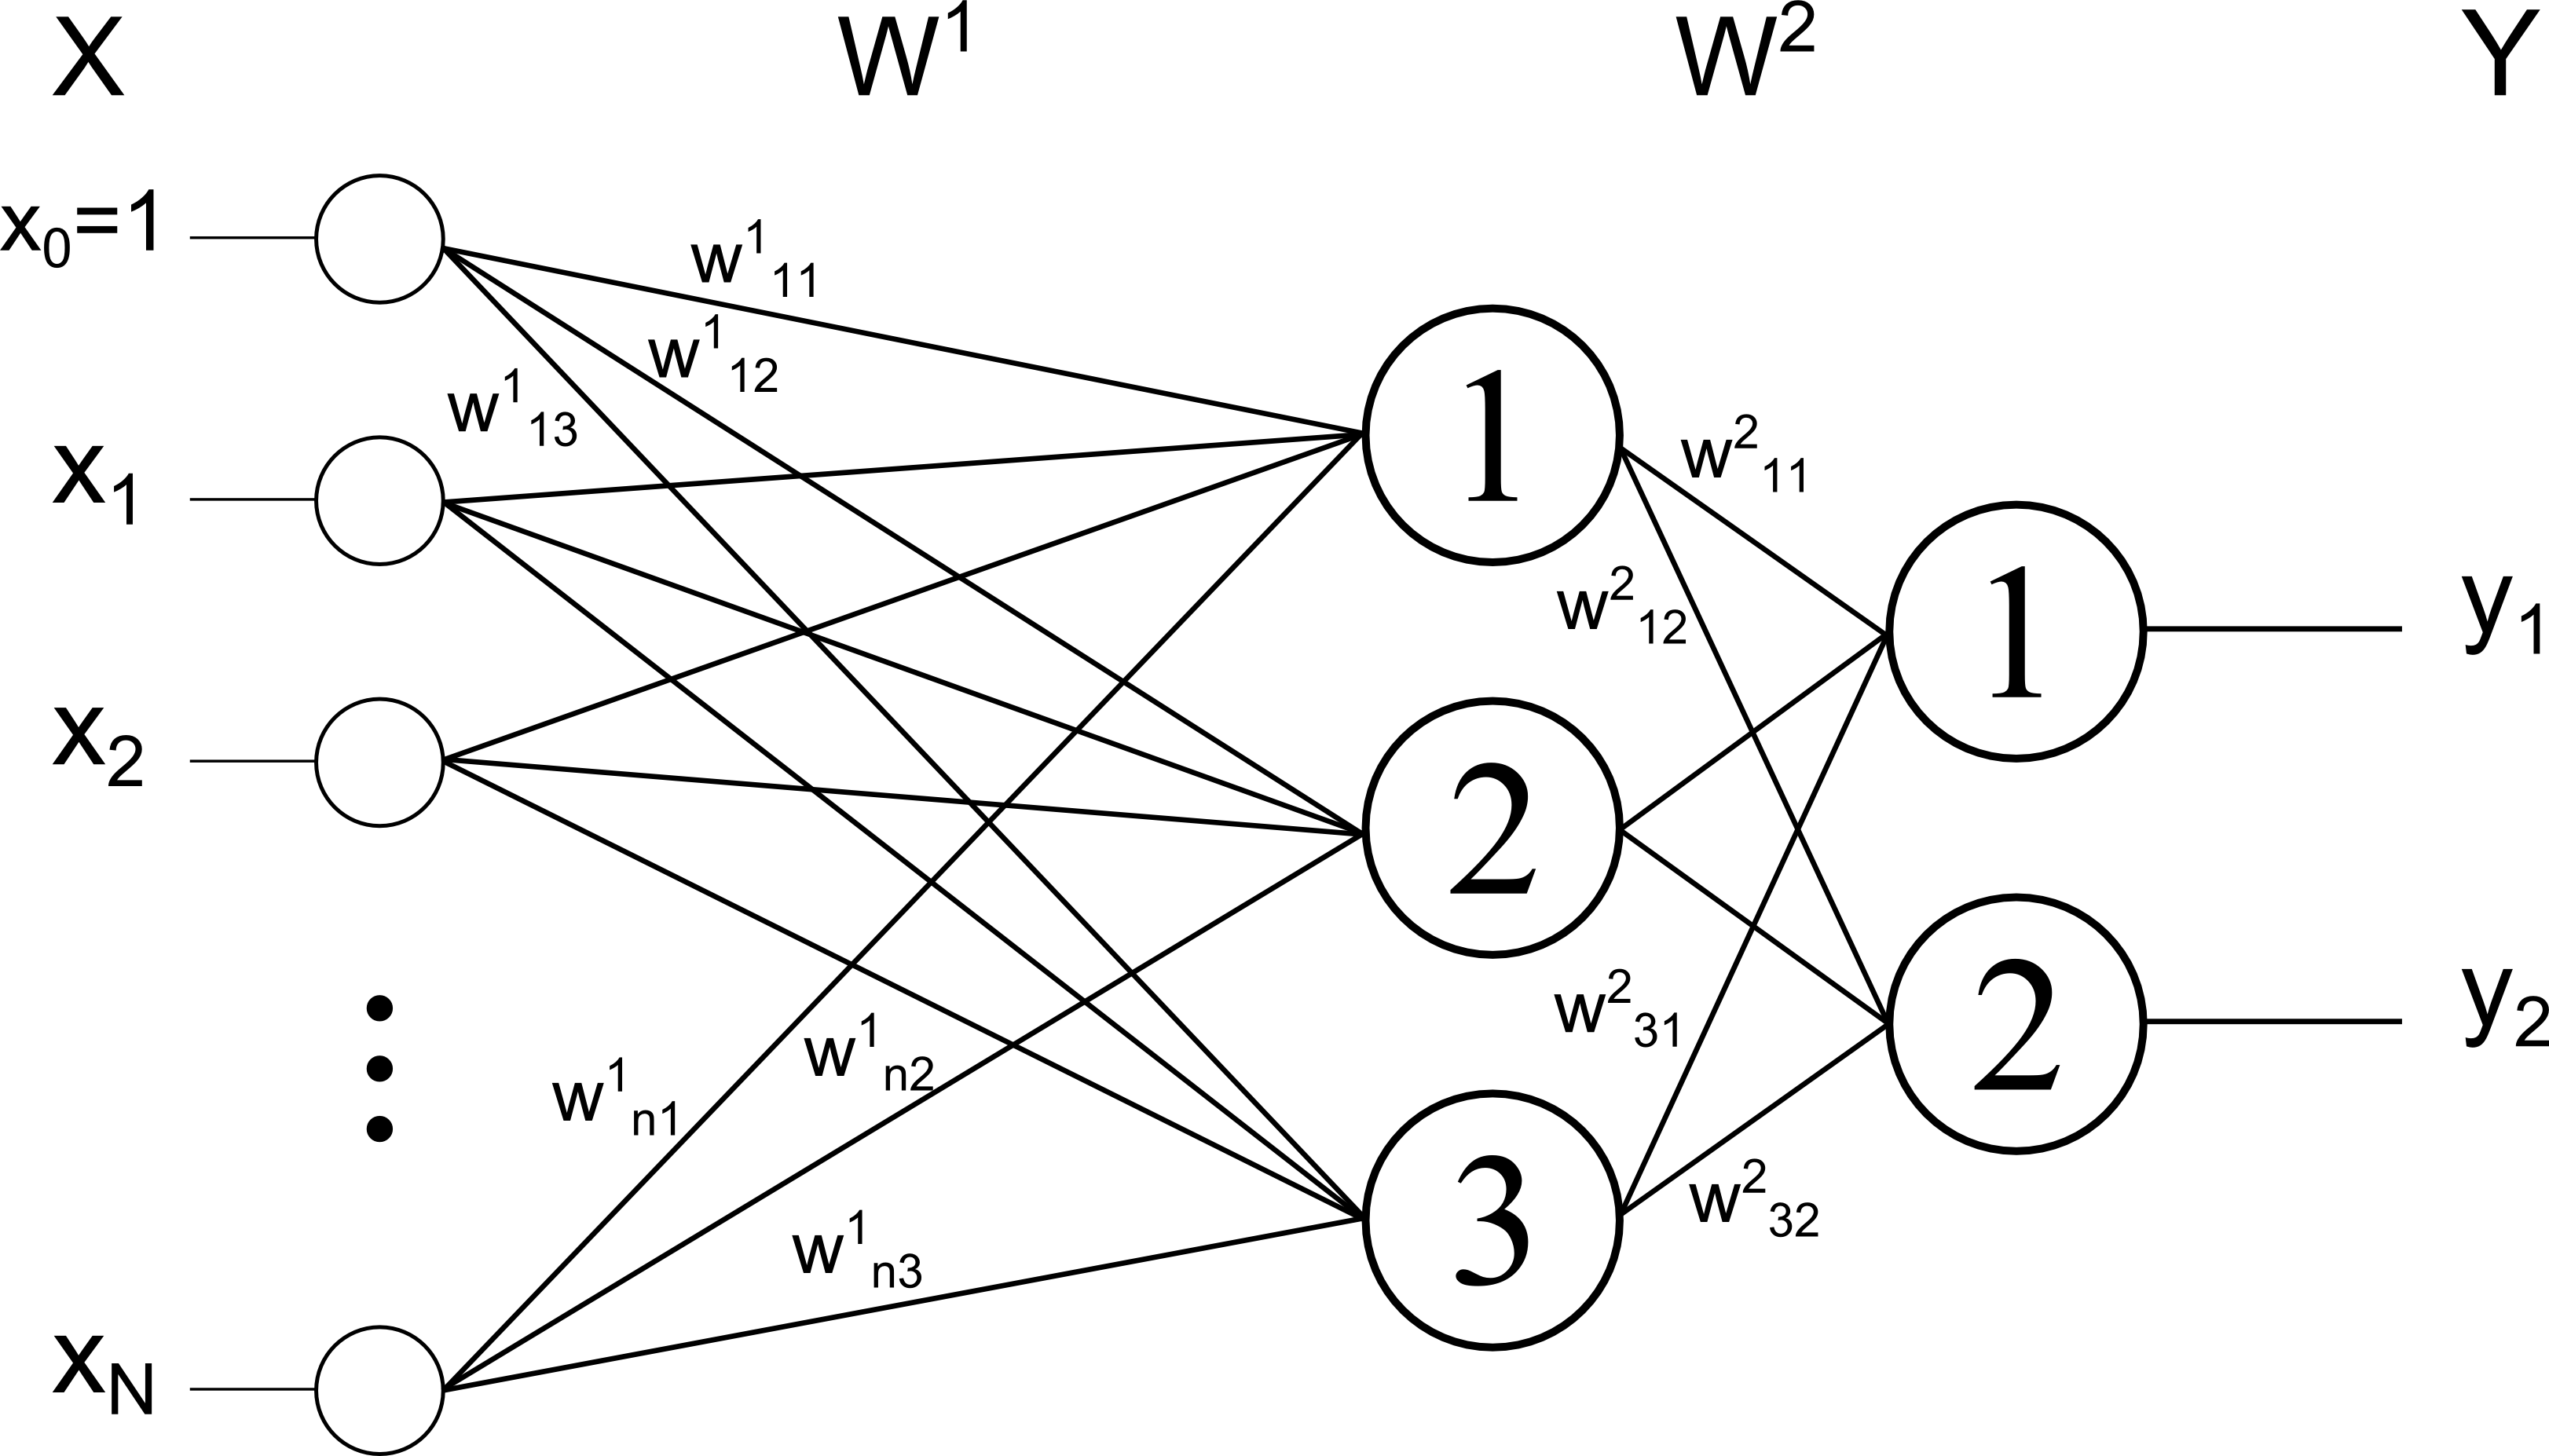
\includegraphics[width=14cm]{perceptron2_my.png}
	\caption{Структура используемого двухслойного персептрона}
	\label{fig:perceptron2_my}
\end{figure}

Для двухслойного персептрона сначала подбиралось количество итераций обучения и скорость обучения при фиксированном размере пачки, равному 600 записей.
Результаты подбора приведены в таблице \ref{tab:mlp2_bf_iter_pace}, оптимальное значение выделено жирным.

\begin{table}[h]
	\centering
	\caption{Подбор количества итераций и скорости обучения для двухслойного персептрона, в таблице указан процент неправильных распознаваний}
	\label{tab:mlp2_bf_iter_pace}
	\begin{tabular}{| l | c | c | c | c | c | c | c | c | c | c |}
		\hline
		Скорость & \multicolumn{6}{c|}{Количество итераций} \\
		\hhline{~----------}
		обучения \phantom{00} & \phantom{00} 100 \phantom{00} & \phantom{0} 1000 \phantom{0} & \phantom{0} 3000 \phantom{0} & \phantom{0} 10000 \phantom{0} & \phantom{0} 30000 \phantom{0} & \phantom{0} 100000 \phantom{0} \\
		\hline
		0.00001  & 94.72 & 95.20 & 92.48 & 77.56 & 47.65 & 37.96 \\
		0.00003  & 95.22 & 92.02 & 82.61 & 59.42 & 38.57 & 33.31 \\
		0.0001 	 & 94.45 & 82.58 & 58.62 & 39.54 & 31.09 & 25.71 \\
		0.0003	 & 93.14 & 56.03 & 46.72 & 35.81 & 30.91 & 22.67 \\
		0.001	 & 83.44 & 47.75 & 40.83 & 30.78 & \textbf{25.34} & 20.51 \\
		0.003	 & 62.90 & 51.70 & 43.55 & 28.81 & 31.67 & 31.84 \\
		0.01	 & 79.46 & 74.27 & 52.63 & 55.74 & 75.28 & 89.29 \\
		0.03	 & 94.19 & 93.45 & 91.46 & 93.58 & 94.33 & 94.16 \\
		0.1		 & 94.13 & 94.26 & 94.61 & 95.01 & 94.98 & 94.47 \\
		0.3		 & 94.43 & 94.80 & 95.03 & 95.02 & 94.87 & 94.97 \\
		1		 & 94.98 & 95.11 & 95.03 & 95.06 & 94.88 & 95.02 \\
		\hline
	\end{tabular}
\end{table}

Оптимальное количество итераций равно 30000, а оптимальная скорость обучения --- 0.001.

Затем подбиралось количество итераций обучения и коэффициент регуляризации при фиксированной скорости обучения, равной 0.001.
Результаты подбора приведены в таблице \ref{tab:mlp2_bf_iter_reg}, оптимальное значение выделено жирным.

\begin{table}[h]
	\centering
	\caption{Подбор количества итераций и коэффициента регуляризации для двухслойного персептрона, в таблице указан процент неправильных распознаваний}
	\label{tab:mlp2_bf_iter_reg}
	\begin{tabular}{| l | c | c | c | c | c | c | c | c | c | c |}
		\hline
		Коэффициент	  & \multicolumn{6}{c|}{Количество итераций} \\
		\hhline{~----------}
		регуляризации & \phantom{0} 100 \phantom{0} & \phantom{0} 1000 \phantom{0} & \phantom{0} 3000 \phantom{0} & \phantom{0} 10000 \phantom{0} & \phantom{0} 30000 \phantom{0} & \phantom{0} 100000 \phantom{0} \\
		\hline
		0.3			  & 89.67 & 92.68 & 87.50 & 79.63 & 79.77 & 77.44 \\
		0.4			  & 85.86 & 88.99 & 83.71 & 71.69 & 66.40 & 66.41 \\
		0.5			  & 85.46 & 87.27 & 84.37 & 65.18 & 56.98 & 56.42 \\
		0.6			  & 85.40 & 86.56 & 78.40 & 59.11 & 52.15 & 48.66 \\
		0.7			  & 83.28 & 80.97 & 78.42 & 51.52 & 42.78 & 38.91 \\
		0.8			  & 80.65 & 72.03 & 67.75 & 42.64 & 36.27 & 32.67 \\
		0.9			  & 83.71 & 46.72 & 41.38 & 33.38 & \textbf{23.30} & 20.03 \\
		1.0			  & 85.23 & 51.60 & 48.78 & 46.84 & 48.14 & 40.41 \\
		\hline
	\end{tabular}
\end{table}

Оптимальное количество итераций равно 30000, а оптимальный коэффициент регуляризации --- 0.9.

Оптимальными параметрами нейронной сети стали: количество итераций обучения --- 30000, скорость обучения --- 0.001, размер пачки 600 и коэффициент регуляризации --- 0.9.
Результаты распознаваний для двухслойного персептрона приведены в таблице \ref{tab:mlp2_dictor1} для случая обучения на наборе данных, состоящем из записей одного диктора, и в таблице \ref{tab:mlp2_dictor2} для случая обучения на наборе данных, состоящем из записей двух дикторов.

\begin{table}[h]
	\centering
	\caption{Результаты распознавания слов двухслойным персептроном на обучающем наборе из одного диктора, в таблице указан процент неправильных распознаваний}
	\label{tab:mlp2_dictor1}
	\begin{tabular}{| l | c | c | c | c | c | c | c | c | c |}
		\hline
		Набор & \multicolumn{9}{c|}{Диктор для распознавания} \\
		\hhline{~---------}
		обучения \phantom{0000} & М1      & М2    	 & М4      & М5    	 & М7      & М8    	 & М9      & М12   	 & РД \\
		\hline
		М1		 &  0.00 & 28.00 & 18.50 & 31.83 & 39.50 & 24.83 & 12.83 & 46.00 & 31.33 \\
		М2		 & 38.67 &  0.33 & 34.67 & 33.83 & 43.50 & 36.17 & 38.67 & 31.83 & 35.33 \\
		М4		 & 13.83 & 17.17 &  0.17 & 15.33 & 15.50 & 24.67 & 15.33 & 22.33 &  9.50 \\
		М5		 & 12.50 & 19.33 &  7.33 &  0.00 & 18.50 & 22.00 & 17.67 & 16.50 & 11.17 \\
		М7		 & 28.33 & 34.33 & 12.67 & 33.33 &  0.00 & 62.83 & 39.50 & 48.00 &  3.67 \\
		М8		 & 15.67 & 18.00 & 18.33 & 22.83 & 34.50 &  0.83 & 20.17 & 25.00 & 18.17 \\
		М9		 & 10.00 & 26.00 & 15.50 & 27.50 & 30.00 & 22.67 &  0.00 & 29.33 & 25.33 \\
		М12		 & 37.50 & 23.67 & 38.83 & 35.50 & 33.17 & 28.83 & 38.00 &  0.00 & 27.00 \\
		РД		 & 32.83 & 36.00 & 23.17 & 38.67 & 15.67 & 43.83 & 42.67 & 41.83 &  0.00 \\
		\hline
	\end{tabular}
\end{table}

\begin{table}[h]
	\centering
	\caption{Результаты распознавания слов двухслойным персептроном на обучающем наборе из двух дикторов, в таблице указан процент неправильных распознаваний}
	\label{tab:mlp2_dictor2}
	\begin{tabular}{| l | c | c | c | c | c | c | c | c | c |}
		\hline
		Набор & \multicolumn{9}{c|}{Диктор для распознавания} \\
		\hhline{~---------}
		обучения \phantom{0000} & М1      & М2    	 & М4      & М5    	 & М7      & М8    	 & М9      & М12   	 & РД \\
		\hline
		М1,М2	 &  3.00 &  3.83 & 17.83 & 24.83 & 34.50 & 21.17 & 25.50 & 40.33 & 31.50 \\
		М2,М4	 &  7.83 &  4.83 &  3.33 & 20.50 & 21.50 & 17.17 & 13.17 & 27.33 & 17.83 \\
		М4,М5	 & 18.17 & 21.33 &  2.33 &  1.83 & 23.50 & 17.33 & 18.17 & 21.33 & 16.83 \\
		М5,М7	 & 14.00 & 13.50 &  7.33 &  2.50 &  3.00 & 18.50 & 21.67 & 18.33 & 11.00 \\
		М7,М8	 & 12.00 & 19.83 &  9.50 & 16.17 &  2.83 &  5.17 & 20.83 & 16.67 &  4.17 \\
		М8,М9	 &  7.17 & 17.67 &  7.50 & 10.33 & 28.00 &  1.83 &  2.33 & 16.33 & 21.83 \\
		М9,М12	 & 13.17 & 26.33 & 14.00 & 20.17 & 25.17 & 21.83 &  4.00 &  3.67 & 14.83 \\
		М12,РД	 & 19.33 & 15.83 & 16.00 & 15.33 & 15.17 & 19.67 & 25.33 &  2.33 &  0.33 \\
		\hline
	\end{tabular}
\end{table}

Среднее количество ошибок при распознавании записей, не входящих в обучающий набор, равно 26.99~\% для первого случая и 18.43~\% для второго.

В итоге, можно сказать, что одно- и двухслойные персептроны показали неудовлетворительные результаты распознавания, с количеством ошибок в несколько раз больше, чем в ранее приведённых алгоритмах.
Далее в разделе будут рассмотрены более подходящие алгоритмы.

\clearpage

%\newpage
%============================================================================================================================

\section{Разработка структур свёрточных сетей глубокого обучения для распознавания речевых команд} \label{sect4_2}

После этого происходил выбор новых архитектур искусственных нейронных сетей, преимущественно среди рекуррентных сетей и сетей глубокого обучения, которые наиболее подходят для задач распознавания речи.
Выбраны свёрточные нейронные сети глубокого обучения.

Итоговая используемая архитектура имеет по 2 слоя свёртки и подвыборки, за которыми идут 3 полносвязных слоя.
Между полносвязными слоями производится регуляризация, состоящая в случайном выбрасывании определённого количества нейронов в процессе обучения.
Такой приём, также, как и в случае многослойных персептронов, улучшает работу сети, предотвращает переобучение и повышает стабильность результатов.
Структура нейронной сети представлена на рисунке \ref{fig:cnn_my}.

\begin{figure}[h]
	\centering
	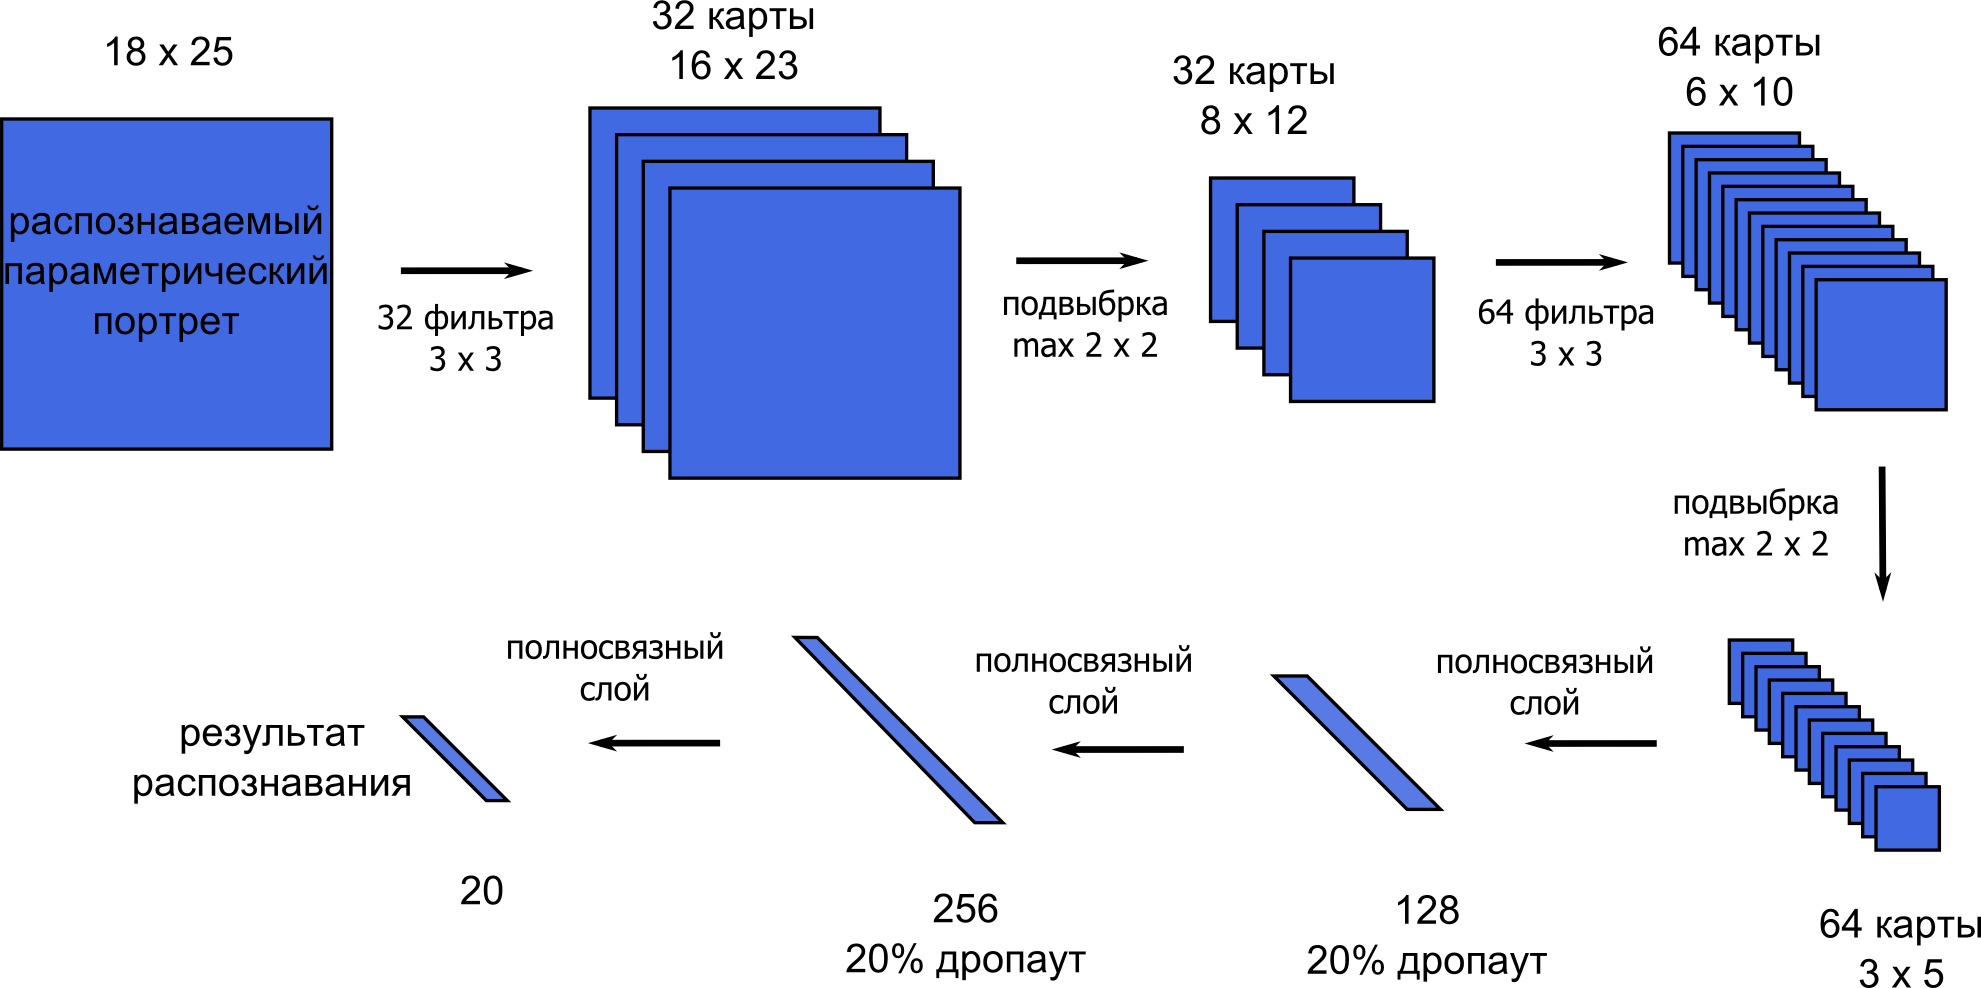
\includegraphics[width=1.0\textwidth]{cnn_my.png}
	\caption{Архитектура используемой свёрточной нейронной сети}
	\label{fig:cnn_my}
\end{figure}

Входной массив является двумерным параметрическим портретом.
Теперь, в отличии от однослойных и многослойных персептронов, нет необходимости преобразовывать двумерный параметрический портрет в одномерный массив.
Далее идёт свёрточный слой с 32 свёрточными фильтрами размером $3 \times 3$.
Затем следует слой подвыборки с размером ядра 2, то есть каждый участок каждой карты признаков размером $2 \times 2$ преобразуется в один элемент в новой карте признаков.
После этого идёт свёрточный слой с 64 фильтрами, каждый из которых применяется ко всем картам признаков и на выходе этого слоя получается 64 карты признаков.
Далее ещё один слой подвыборки с размером ядра 2, за которым идут три полносвязных слоя со 128, 256 и 20 элементами соответственно, где 20 --- это количество распознаваемых слов.
Таким образом, общее количество параметров данной нейронной сети равно $(3 \times 3 \times 1 + 1) \times 32 + (3 \times 3 \times 32 + 1)  \times 64 + (64 \times 3 \times 5 + 1) \times 128 + (128 + 1) \times 256 + (256 + 1) \times 20 = 179 988$.

В свёрточных слоях, также, как и многослойных персепронах, используется функция активации ReLU.
В первых двух полносвязных слоях используется гиперболический тангенс в качестве функции активации, который задаётся уравнением $f(x) = \tanh(x) = \frac{e^x - e^{-x}}{e^x + e^{-x}}$.
Также, после обоих скрытых полносвязных слоев применяется регуляризация для предотвращения переобучения сети.
Для последнего полносвязного слоя используется функция softmax для нормировки полученных выходных вероятностей.
Для обучения данного типа нейронных сетей в качестве функции потерь используется перекрёстная энтропия.
В процессе обучения используется вариант оптимизации Adam для стохастического градиентного спуска.

Приведённые выше количество и размеры фильтров, а также размеры финальных полносвязных слоев взяты из эмпирических рекомендаций для распознавания изображений свёрточными нейронными сетями.
Параметрический портрет является своего рода изображением, поэтому было решено использовать аналогичные параметры.

Важным является вопрос использования свёрточных нейронных сетей для малых обучающих выборок, размер которых в нашем случае будет составлять от 300 до 4900 записей.
Также стоит отметить небольшое количество классов: 20 для распознавания слов и 11 для распознавания фраз.
При этом количество элементов каждого класса в обучающей выборке не меньше 30.

Хотя изначально свёрточные нейронные сети обучались на больших выборках, в последнее время были получены обнадёживающие результаты на обучающих выборках небольшого размера.
Например, в работе \cite{dieleman2015classifying} использовалось 27000 элементов из 121 несбалансированного класса для распознавания изображений, а в работе \cite{truong2018lightweight} была использована база данных CIFAR-10 \cite{cifar10} c 50000 элементами из 10 классов в обучающей выборке.
При этом, при соблюдении определённых условий свёрточные нейронные сети показывают хорошие результаты при обучении на маленьких выборках, размером 100--1000 элементов, даже при количестве обучаемых параметров порядка нескольких сотен тысяч \cite{beam2017cnn}.
Количество обновлений градиента на одной итерации равно числу элементов в обучающей выборке, следовательно, необходимо уделить особое внимание количеству итераций и убедиться в сходимости процесса обучения.
Рекомендуется использовать функцию активации ReLU для более быстрого схождения процесса обучения и различные способы регуляризации для предотвращения переобучения.
Все указанные рекомендации были применены в используемой свёрточной нейронной сети, что даёт позволило надеяться на хороший результат.

Был произведён подбор параметров модели и выбор оптимальной сети на небольшой обучающей выборке при распознавании фраз вне этой выборки.
Подбирались оптимальные значения для количества итераций обучения и скорость обучения при фиксированном размере пачки, равному 600 записей.
Результаты подбора приведены в таблице \ref{tab:cnn_bf_iter_pace}, оптимальное значение выделено жирным.

\begin{table}[h]
	\centering
	\caption{Подбор количества итераций и скорости обучения для свёрточной нейронной сети при распознавании слов, в таблице указан процент неправильных распознаваний}
	\label{tab:cnn_bf_iter_pace}
	\begin{tabular}{| l | c | c | c | c | c | c |}
		\hline
		Скорость & \multicolumn{5}{c|}{Количество итераций} \\
		\hhline{~-----}
		обучения \phantom{00} & \phantom{000} 100 \phantom{000} & \phantom{000}1000\phantom{000} & \phantom{000}3000\phantom{000} & \phantom{00} 10000 \phantom{00} & \phantom{00} 30000 \phantom{00} \\
		\hline
		0.00001	& 70.70 & 22.60 & 13.50 &  9.50 &  7.50 \\
		0.00003	& 42.10 & 13.20 &  9.00 &  7.10 &  6.50 \\
		0.0001	& 28.50 &  9.20 &  7.20 &  6.30 &  6.00 \\
		0.0003	& 20.60 &  7.70 &  6.50 & \textbf{5.30} &  6.10 \\
		0.001	& 44.00 &  8.40 &  8.10 &  8.30 &  8.80 \\
		0.003	& 84.00 & 10.80 &  9.10 & 11.70 & 11.20 \\
		0.01	& 94.20 & 52.90 & 43.20 & \multicolumn{1}{c|}{---} & \multicolumn{1}{c|}{---} \\	
		0.03	& 95.10 & 94.90 & 94.90 & \multicolumn{1}{c|}{---} & \multicolumn{1}{c|}{---} \\	
		0.1		& 95.00 & 95.00 & 95.00 & \multicolumn{1}{c|}{---} & \multicolumn{1}{c|}{---} \\
		\hline
	\end{tabular}
\end{table}

Оптимальными параметрами нейронной сети стали: количество итераций обучения --- 10000, скорость обучения --- 0.0003 и размер пачки 600.
Результаты распознаваний для свёрточной нейронной сети на одном и нескольких дикторах приведены ниже.

%\newpage
%============================================================================================================================

\section{Экспериментальное оценивание характеристик распознавания свёрточной нейронной сети глубокого обучения} \label{sect4_3}

Проведён следующий эксперимент.
Записи каждого диктора разбивались на 2 части.
На первой части обучалась свёрточная нейронная сеть, а вторая часть использовалась в качестве тестовой выборки.
Результаты этих распознаваний приведены на рисунке \ref{fig:cnn_words_self}.
В столбцах отложено количество записей для каждого слова, содержащихся в обучающей выборке.
В строках указан диктор, для которого проводилось обучение и распознавание.

\begin{figure}[h]
	\centering
	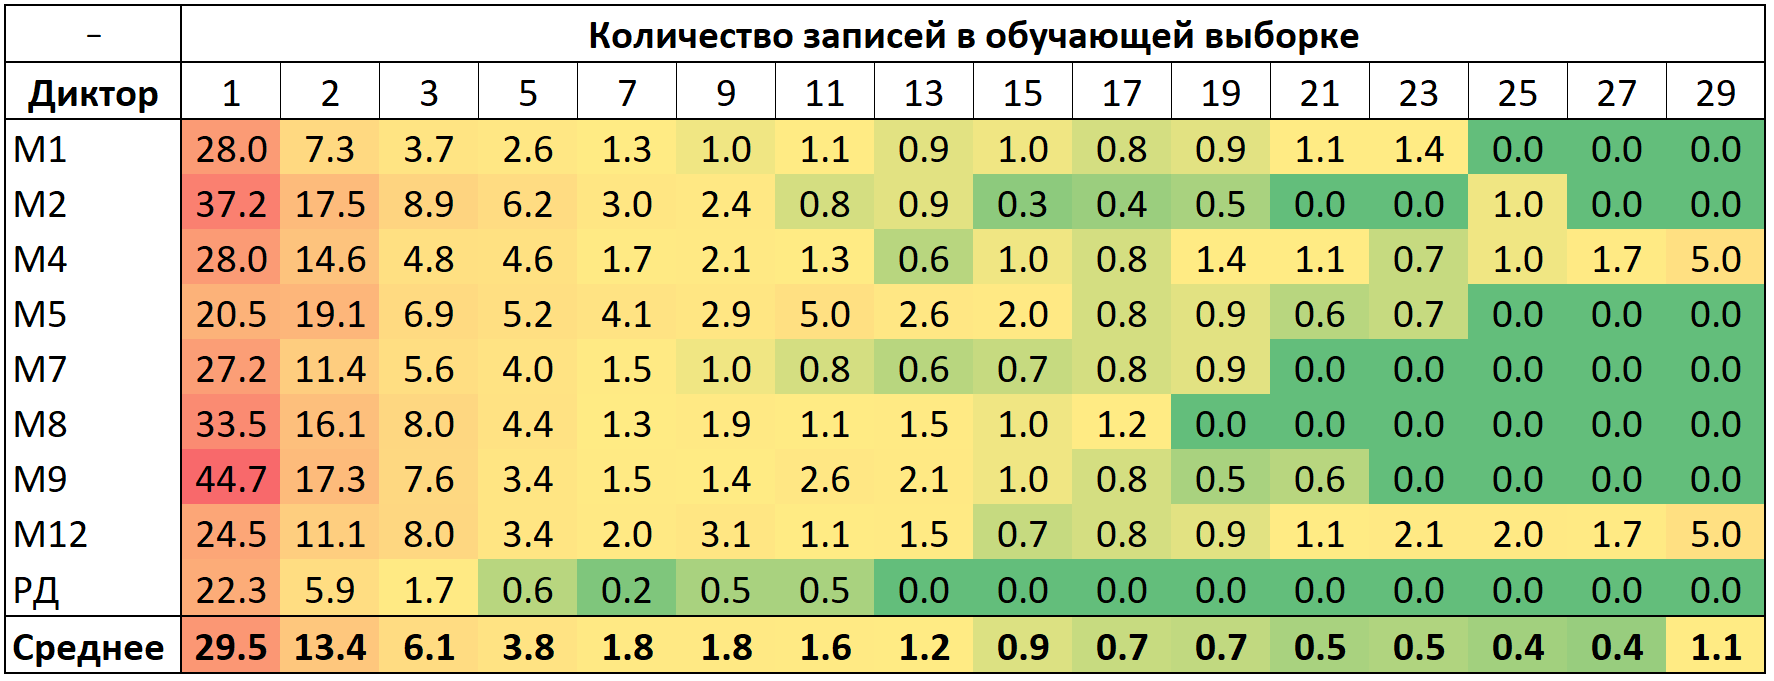
\includegraphics[width=1.0\textwidth]{cnn_words_self.png}
	\caption{Результаты распознавания слов свёрточной нейронной сетью при обучении на том же дикторе, в таблице указан процент неправильных распознаваний}
	\label{fig:cnn_words_self}
\end{figure}

Видно, что достаточно обучиться на 7 записях, чтобы ошибка стала ниже 2~\%, на 15 записях, чтобы стала ниже 1~\% и на 21 записи для 0.5~\% ошибок.
Данные результаты показывают, к каким величинам ошибок нужно стремиться при распознавании записей других дикторов для исключения эффекта дикторозависимости.

После этого проводилось распознавание с помощью одного диктора.
Это означает, что нейронная сеть обучалась на записях одного диктора и затем записи всех дикторов распознавались на этой нейронной сети.
При распознавании слов из обучающей выборки в среднем получается 0.0~\% ошибок, а для распознавания слов из тестовой выборки --- 5.9~\% ошибок.
Подробные результаты приведены в таблице \ref{tab:cnn_1dictor}.

\begin{table}[h]
	\centering
	\caption{Результаты распознавания слов свёрточной нейронной сетью на обучающем наборе из одного диктора в условиях без шума, в таблице указан процент неправильных распознаваний}
	\label{tab:cnn_1dictor}
	\begin{tabular}{| l | c | c | c | c | c | c | c | c | c |}
		\hline
		Набор & \multicolumn{9}{c|}{Диктор для распознавания} \\
		\hhline{~---------}
		обучения \phantom{00} & \phantom{0}М1\phantom{0} & \phantom{0}М2\phantom{0} & \phantom{0}М4\phantom{0} & \phantom{0}М5\phantom{0} & \phantom{0}М7\phantom{0} & \phantom{0}М8\phantom{0} & \phantom{0}М9\phantom{0} & \phantom{0}М12\phantom{0} & \phantom{0}РД\phantom{0} \\
		\hline
		М1		 & 0.0 & 6.3 & 2.5 & 7.7 &  7.8 &  8.2 &  2.5 &  4.7 & 5.3 \\
		М2		 & 1.7 & 0.0 & 0.7 & 3.3 &  2.7 &  9.5 &  6.0 &  8.3 & 1.0 \\
		М4		 & 2.7 & 6.2 & 0.2 & 3.0 &  3.0 &  5.3 &  5.0 &  6.8 & 0.8 \\
		М5		 & 6.2 & 7.8 & 2.0 & 0.0 &  7.3 &  6.0 &  6.5 &  2.8 & 3.3 \\
		М7		 & 9.5 & 7.8 & 2.3 & 5.5 &  0.0 & 22.0 & 10.3 & 24.5 & 3.7 \\
		М8		 & 4.5 & 4.7 & 2.8 & 3.3 & 10.0 &  0.0 &  6.3 &  2.5 & 3.0 \\
		М9		 & 2.3 & 6.7 & 3.7 & 3.7 &  7.5 &  7.8 &  0.0 &  7.5 & 2.7 \\
		М12		 & 5.2 & 7.3 & 6.0 & 4.7 &  9.2 &  6.3 &  8.0 &  0.0 & 3.8 \\
		РД		 & 7.2 & 7.7 & 4.0 & 4.7 &  2.5 &  9.3 & 11.3 & 13.2 & 0.0 \\
		\hline
	\end{tabular}
\end{table}

Далее было проведено распознавание с помощью трёх дикторов.
При распознавании слов из обучающей выборки в среднем получается 0.0~\% ошибок, а для распознавания слов из тестовой выборки --- 1.7~\% ошибок.
Подробные результаты приведены в таблице \ref{tab:cnn_3dictor}.

\begin{table}[h]
	\centering
	\caption{Результаты распознавания слов свёрточной нейронной сетью на обучающем наборе из трёх дикторов в условиях без шума, в таблице указан процент неправильных распознаваний}
	\label{tab:cnn_3dictor}
	\begin{tabular}{| l | c | c | c | c | c | c | c | c | c |}
		\hline
		Набор & \multicolumn{9}{c|}{Диктор для распознавания} \\
		\hhline{~---------}
		обучения  & \phantom{0}М1\phantom{0} & \phantom{0}М2\phantom{0} & \phantom{0}М4\phantom{0} & \phantom{0}М5\phantom{0} & \phantom{0}М7\phantom{0} & \phantom{0}М8\phantom{0} & \phantom{0}М9\phantom{0} & \phantom{0}М12\phantom{0} & \phantom{0}РД\phantom{0} \\
		\hline
		М1,М2,М4  & 0.0 & 0.0 & 0.2 & 2.3 & 0.7 & 3.7 & 2.0 & 2.7 & 0.7 \\
		М2,М4,М5  & 1.7 & 0.0 & 0.2 & 0.0 & 1.3 & 3.2 & 1.7 & 1.7 & 0.2 \\
		М4,М5,М7  & 2.3 & 2.2 & 0.2 & 0.0 & 0.0 & 3.3 & 1.7 & 4.0 & 0.3 \\
		М5,М7,М8  & 2.0 & 2.3 & 0.7 & 0.0 & 0.0 & 0.0 & 1.8 & 1.3 & 0.7 \\
		М7,М8,М9  & 1.3 & 1.7 & 0.7 & 1.0 & 0.0 & 0.0 & 0.0 & 1.8 & 0.0 \\
		М8,М9,М12 & 1.7 & 3.3 & 0.8 & 0.5 & 2.7 & 0.0 & 0.0 & 0.0 & 1.0 \\
		М9,М12,РД & 1.7 & 3.8 & 0.5 & 1.3 & 1.2 & 2.5 & 0.0 & 0.0 & 0.0 \\
		М12,РД,М1 & 0.0 & 2.3 & 0.5 & 1.2 & 2.0 & 1.7 & 1.8 & 0.0 & 0.0 \\
		РД,М1,М2  & 0.0 & 0.0 & 0.3 & 1.5 & 0.7 & 3.0 & 2.0 & 2.2 & 0.0 \\
		\hline
	\end{tabular}
\end{table}

Для распознавания большим числом дикторов были составлены несколько наборов данных для обучения.
Каждый набор состоит из записей слов 7 различных дикторов.
Далее на нейронных сетях, обученных на составленных наборах, производились распознавания на обучающей и тестовой выборках.
В таблице \ref{tab:cnn_without_noise} приведены результаты описанных распознаваний.

\begin{table}[h]
	\centering
	\caption{Результаты распознавания слов для случая записей без шума при распознавании на обучающем наборе из семи дикторов, в таблице указан процент неправильных распознаваний}
	\label{tab:cnn_without_noise}
	\begin{tabular}{| l | c | c | c | c | c | c | c | c | c |}
		\hline
		 & \multicolumn{9}{c|}{Диктор для распознавания} \\
		\hhline{----------}
		Набор обучения \phantom{0000000000000} & М1  & М2  & М4  & М5  & М7  & М8  & М9  & М12 & РД \\
		\hline
		М1,М2,М4,М5,М7,М8,М9  & 0.0 & 0.0 & 0.2 & 0.0 & 0.0 & 0.0 & 0.0 & 0.5 & 0.0 \\
		М2,М4,М5,М7,М8,М9,М12 & 0.8 & 0.0 & 0.2 & 0.0 & 0.0 & 0.0 & 0.0 & 0.0 & 0.0 \\
		М4,М5,М7,М8,М9,М12,РД & 1.2 & 1.2 & 0.2 & 0.0 & 0.0 & 0.0 & 0.0 & 0.0 & 0.0 \\
		М5,М7,М8,М9,М12,РД,М1 & 0.0 & 1.2 & 0.2 & 0.0 & 0.0 & 0.0 & 0.0 & 0.0 & 0.0 \\
		М7,М8,М9,М12,РД,М1,М2 & 0.0 & 0.0 & 0.5 & 0.5 & 0.0 & 0.0 & 0.0 & 0.0 & 0.0 \\
		М8,М9,М12,РД,М1,М2,М4 & 0.0 & 0.0 & 0.2 & 0.3 & 0.3 & 0.0 & 0.0 & 0.0 & 0.0 \\
		М9,М12,РД,М1,М2,М4,М5 & 0.0 & 0.0 & 0.2 & 0.0 & 0.7 & 1.2 & 0.0 & 0.0 & 0.0 \\
		М12,РД,М1,М2,М4,М5,М7 & 0.0 & 0.0 & 0.2 & 0.0 & 0.0 & 1.5 & 0.5 & 0.0 & 0.0 \\
		РД,М1,М2,М4,М5,М7,М8  & 0.0 & 0.0 & 0.2 & 0.0 & 0.0 & 0.0 & 0.7 & 0.5 & 0.0 \\
		\hline
	\end{tabular}
\end{table}

При распознавании слов из обучающей выборки ошибок нет, а для распознавания слов из тестовой выборки в среднем получается 0.6~\% ошибок.

В таблице \ref{tab:cnn_without_noise_summary} приведены суммарные результаты распознавания записей без шума при обучении на различном числе дикторов.

\begin{table}[h]
	\centering
	\caption{Суммарные результаты распознаваний слов на обучающих наборах из различного количества дикторов для случая записей без шума}
	\label{tab:cnn_without_noise_summary}
	\begin{tabular}{| l | c | c | c | c | c | c | c |}
		\hline
		Количество дикторов	\phantom{000} & \phantom{00}1\phantom{00} & \phantom{00}2\phantom{00} & \phantom{00}3\phantom{00} & \phantom{00}4\phantom{00} & \phantom{00}5\phantom{00} & \phantom{00}6\phantom{00} & \phantom{00}7\phantom{00} \\
		\hline
		Процент ошибок		& 5.9 & 2.4 & 1.7 & 1.2 & 1.0 & 0.8 & 0.6 \\
		\hline
	\end{tabular}
\end{table}

Из результатов можно сделать вывод, что процент ошибок стабильно снижается при увеличении количества дикторов в обучающей базе.
Большее число дикторов позволяет избавиться от дикторозависимости, что положительно сказывается на качестве распознавания.

\clearpage

%\newpage
%============================================================================================================================

\section{Обучение и тестирование свёрточной нейронной сети глубокого обучения на данных содержащих шум кабины пилотов современного магистрального самолёта} \label{sect4_4}

В данном подразделе приведены результаты распознавания записей в условиях шума.
Шум моделировался следующим образом.
Для каждой записи выбирались уникальные отрезки шума из записи шума кабины самолёта Boeing со средней громкостью более 80 дБ.
При этом громкость шума нормировалась так, чтобы отношение сигнал/шум было равно некоторой фиксированной величине.

Проведён эксперимент по распознаванию записей того же диктора, записи которого использовались в качестве обучающей выборки.
Также как и случае записей без шума, записи каждого диктора разбивались на 2 части: на первой части обучалась свёрточная нейронная сеть, а вторая часть использовалась в качестве тестовой выборки.
Результаты этих распознаваний приведены на рисунке \ref{fig:cnn_words_self_noise}.
По столбцам отложено количество записей для каждого слова, содержащихся в обучающей выборке.
В столбцах указан уровень наложенного шума.
Приведённые результаты являются усреднёнными значениями по всем дикторам.

\begin{figure}[h]
	\centering
	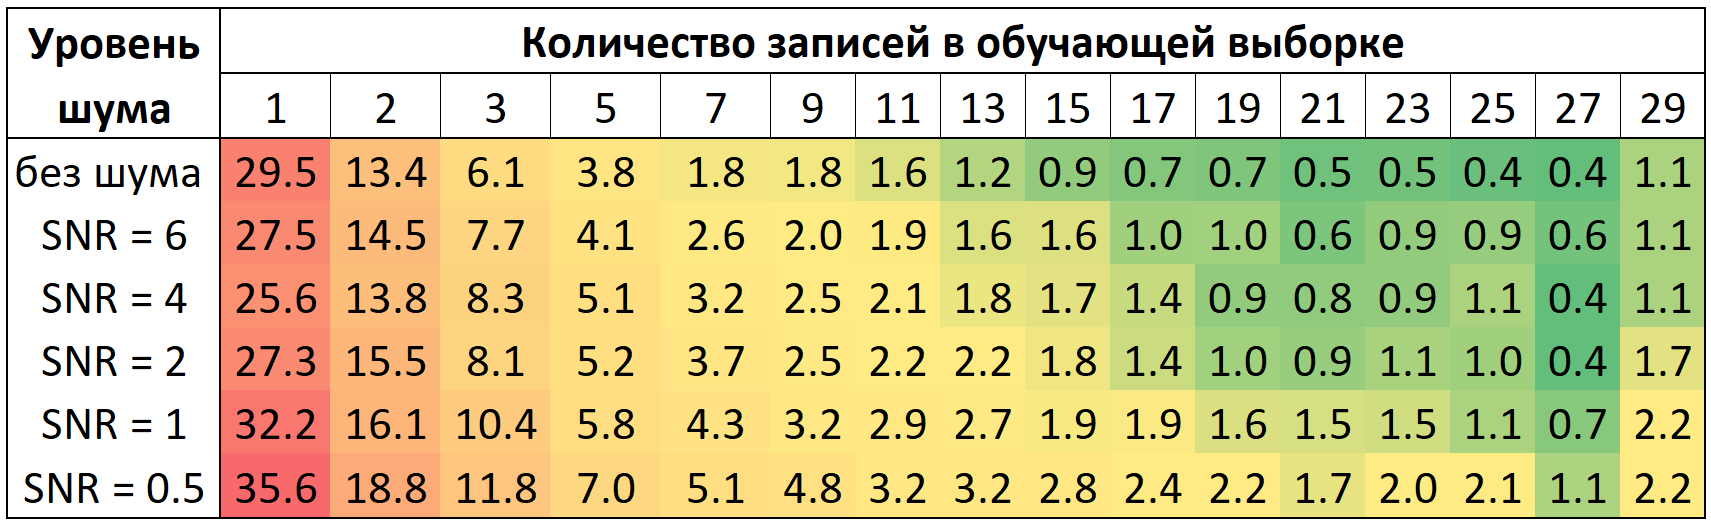
\includegraphics[width=1.0\textwidth]{cnn_words_self_noise.png}
	\caption{Усреднённые результаты распознавания слов свёрточной нейронной сетью в условиях различных уровней шума при обучении на том же дикторе, в таблице указан процент неправильных распознаваний}
	\label{fig:cnn_words_self_noise}
\end{figure}

Видно, что результаты монотонно ухудшаются с увеличением уровня шума, при этом по величине ухудшение оказывается незначительным.
Например, при использовании 15 записей в обучающей выборке при отсутствии шума получается 0.9~\% ошибок, а при отношении сигнал/шум равном 1 получается 1.9~\% ошибок.
Аналогичные значения при обучении на 9 записях равны 1.8 и 3.2~\% соответственно.
Данные результаты показывают, к каким величинам ошибок нужно стремиться при распознавании записей с шумом других дикторов для исключения эффекта дикторозависимости.

После этого было проведено обычное распознавание одним диктором с наложением одного варианта шума.
Здесь и далее громкость шума нормировалась так, чтобы отношение сигнал/шум было равно 4.
Для увеличения обучающей выборки и улучшения процесса обучения на записи могут накладываться различные уникальные варианты шума.
В таблице \ref{tab:cnn_1noise_1dictor} представлено 2 варианта эксперимента.
В первом случае обучение проводилось на записях с шумом, а распознавались записи без шума.

\begin{table}[h]
	\centering
	\caption{Результаты распознавания слов для случая записей с шумом при распознавании на обучающем наборе из одного диктора, в таблице указан процент неправильных распознаваний}
	\label{tab:cnn_1noise_1dictor}
	\begin{tabular}{| l | c | c | c | c | c | c | c | c | c |}
		\hline
		Набор & \multicolumn{9}{c|}{Диктор для распознавания} \\
		\hhline{~---------}
		обучения\phantom{00} & \phantom{0}М1\phantom{0} & \phantom{0}М2\phantom{0} & \phantom{0}М4\phantom{0} & \phantom{0}М5\phantom{0} & \phantom{0}М7\phantom{0} & \phantom{0}М8\phantom{0} & \phantom{0}М9\phantom{0} & \phantom{0}М12\phantom{0} & \phantom{0}РД\phantom{0} \\
		\hline
		\multicolumn{10}{|c|}{обучение с шумом, распознавание без шума} \\
		\hline
		М1		 &  0.0 & 13.8 &  6.3 & 12.2 & 11.7 & 14.8 &  9.3 & 16.7 &  9.0 \\
		М2		 &  7.2 &  0.2 & 15.8 & 12.0 & 27.7 & 10.0 & 18.3 &  9.2 & 11.5 \\
		М4		 &  5.8 &  7.0 &  0.3 & 10.0 &  6.5 & 10.3 &  7.3 & 13.2 &  1.3 \\
		М5		 &  7.0 & 10.0 &  3.8 &  0.0 & 13.0 &  7.5 & 11.8 &  4.8 &  8.0 \\
		М7		 & 14.5 & 13.3 &  7.3 & 15.2 &  0.2 & 18.2 & 14.7 & 24.7 &  5.3 \\
		М8		 &  9.2 &  7.8 &  7.7 &  7.5 & 16.3 &  0.0 & 12.2 &  8.7 &  5.2 \\
		М9		 &  5.0 & 11.2 &  8.5 &  9.2 & 14.2 & 11.3 &  0.0 & 14.3 & 10.3 \\
		М12		 & 12.3 & 11.0 & 16.3 & 14.8 & 16.8 & 14.3 & 18.5 &  0.2 &  9.3 \\
		РД		 & 19.7 & 14.8 & 11.5 & 15.2 &  8.7 & 19.5 & 18.7 & 24.2 &  1.7 \\
		\hline
		\multicolumn{10}{|c|}{обучение с шумом, распознавание с шумом} \\
		\hline
		М1		 &  0.0 & 11.2 &  5.7 & 14.0 & 14.2 & 17.0 &  4.3 & 11.8 &  8.3 \\
		М2		 &  3.3 &  0.0 &  2.2 &  5.0 &  8.3 & 11.5 &  7.2 &  8.2 &  1.2 \\
		М4		 &  5.3 & 10.2 &  0.0 & 11.3 &  5.3 & 16.3 &  7.5 & 12.0 &  2.3 \\
		М5		 &  8.0 & 10.2 &  3.3 &  0.0 & 11.5 & 10.2 &  8.5 &  4.7 &  8.2 \\
		М7		 & 11.7 & 12.2 &  5.3 & 11.8 &  0.0 & 26.8 & 12.3 & 25.7 &  0.8 \\
		М8		 &  7.8 &  8.5 &  5.7 &  4.7 & 10.0 &  0.0 & 11.7 &  8.8 &  6.0 \\
		М9		 &  5.3 &  9.3 &  8.2 &  9.2 & 10.3 & 20.2 &  0.0 & 19.5 & 13.2 \\
		М12		 &  8.8 & 11.2 &  7.7 &  8.0 &  8.7 & 14.5 & 10.0 &  0.0 &  6.2 \\
		РД		 & 10.5 & 11.2 &  5.8 & 11.2 &  4.5 & 14.8 & 15.2 & 19.7 &  0.0 \\
		\hline
	\end{tabular}
\end{table}

Средняя ошибка при распознавании записей диктора, на которых проводилось обучение, равна 0.3~\%, а средняя ошибка для записей других дикторов --- 11.8~\%.
Во втором случае и обучение, и распознавание проводилось на записях с шумом.
На записях, на которых проводилось обучение, ошибок не было, а средняя ошибка для записей других дикторов равна 9.7~\%.
Из этих результатов видно, что для обоих вариантов распознавания ошибка получается выше, чем при использовании записей без шума.
Также проводился эксперимент, в котором обучение проводилось на записях без шума, а распознавания на записях с шумом.
Для этого варианта количество ошибок получалось в несколько раз больше, чем для предыдущих, поэтому в дальнейшем такой вариант использоваться не будет.

Далее был проведён аналогичный эксперимент, но с тем отличием, что для обучения использовались записи с семью различными наложенными вариантами шума.
Для первого эксперимента средняя ошибка при распознавании записей диктора, на которых проводилось обучение, равна 0.0~\%, а средняя ошибка для записей других дикторов --- 8.5~\%.
Для второго эксперимента на записях, на которых проводилось обучение, ошибок не было, а средняя ошибка для записей других дикторов равна 8.2~\%.
Как видно из результатов, использование нескольких вариантов шумов заметно улучшает качество распознавания.
Результаты данных экспериментов приведены в таблице \ref{tab:cnn_7noise_1dictor}.

\begin{table}[h]
	\centering
	\caption{Результаты распознавания слов для случая записей с шумом при распознавании на обучающем наборе из одного диктора с 7 вариантами шума, в таблице указан процент неправильных распознаваний}
	\label{tab:cnn_7noise_1dictor}
	\begin{tabular}{| l | c | c | c | c | c | c | c | c | c |}
		\hline
		Набор & \multicolumn{9}{c|}{Диктор для распознавания} \\
		\hhline{~---------}
		обучения\phantom{00} & \phantom{0}М1\phantom{0} & \phantom{0}М2\phantom{0} & \phantom{0}М4\phantom{0} & \phantom{0}М5\phantom{0} & \phantom{0}М7\phantom{0} & \phantom{0}М8\phantom{0} & \phantom{0}М9\phantom{0} & \phantom{0}М12\phantom{0} & \phantom{0}РД\phantom{0} \\
		\hline
		\multicolumn{10}{|c|}{обучение с шумом, распознавание без шума} \\
		\hline
		М1		 &  0.0 & 10.2 &  5.8 & 10.8 & 10.3 & 13.5 &  7.3 & 11.7 & 10.3 \\
		М2		 &  3.7 &  0.0 &  2.5 &  5.0 &  9.2 &  9.5 &  7.8 &  5.2 &  1.2 \\
		М4		 &  4.5 &  7.3 &  0.2 &  6.3 &  5.8 &  8.5 &  8.7 &  9.8 &  2.3 \\
		М5		 &  6.0 &  8.3 &  2.2 &  0.0 &  7.0 &  4.7 &  7.0 &  4.2 &  5.7 \\
		М7		 & 12.2 & 12.3 &  6.0 & 15.5 &  0.0 & 21.2 &  9.3 & 29.0 &  4.3 \\
		М8		 &  6.0 &  5.7 &  3.7 &  3.3 &  7.8 &  0.0 &  9.2 &  8.8 &  4.2 \\
		М9		 &  4.7 & 10.5 &  7.3 &  7.3 & 12.0 &  7.5 &  0.0 & 10.0 & 11.7 \\
		М12		 &  8.7 &  9.8 & 10.8 & 11.0 &  9.2 & 10.0 &  7.5 &  0.0 &  5.2 \\
		РД		 & 13.3 & 10.8 &  5.7 &  8.2 &  4.3 & 12.3 & 15.2 & 19.3 &  0.0 \\
		\hline
		\multicolumn{10}{|c|}{обучение с шумом, распознавание с шумом} \\
		\hline
		М1		 &  0.0 &  8.5 &  4.0 &  9.5 & 13.7 & 13.3 &  3.8 &  8.3 &  7.2 \\
		М2		 &  2.5 &  0.0 &  2.7 &  5.5 &  5.8 & 12.5 &  5.8 &  5.0 &  1.7 \\
		М4		 &  6.0 &  7.3 &  0.0 &  9.5 &  5.2 & 13.3 &  8.3 & 11.3 &  2.0 \\
		М5		 &  5.7 &  8.2 &  1.5 &  0.0 &  7.8 &  7.8 &  7.3 &  4.7 &  4.8 \\
		М7		 & 10.7 & 12.2 &  5.7 & 13.2 &  0.0 & 24.2 & 10.7 & 20.5 &  1.3 \\
		М8		 &  5.0 &  8.2 &  3.3 &  4.2 &  8.2 &  0.0 &  8.7 & 10.7 &  3.8 \\
		М9		 &  4.3 & 10.5 &  5.7 &  6.7 &  7.2 & 15.7 &  0.0 & 13.0 &  6.8 \\
		М12		 &  7.8 & 11.5 &  7.0 &  6.5 &  7.3 & 12.5 &  5.3 &  0.0 &  5.8 \\
		РД		 & 10.8 & 13.5 &  5.3 & 10.5 &  3.5 & 15.5 & 14.3 & 13.5 &  0.0 \\
		\hline
	\end{tabular}
\end{table}

После этого было проведено обучение нейронной сети на 3 дикторах в условиях шума и последующее распознавания записей.
Первый эксперимент предполагает использование одного варианта шума при обучении, а второй эксперимент --- 3 варианта шума.
В обоих случаях средняя величина ошибки при распознавании записей диктора, на которых проводилось обучение, равна 0.0~\%.
Для случая распознавания записей других дикторов ошибка равна 2.8~\% для первого эксперимента и 2.5~\% для второго.
Подробные результаты экспериментов приведены в таблице \ref{tab:cnn_noise_3dictors}.

\begin{table}[h]
	\centering
	\caption{Результаты распознавания слов для случая записей с шумом при распознавании на обучающем наборе из трёх дикторов с 1 и 3 вариантами шума, в таблице указан процент неправильных распознаваний}
	\label{tab:cnn_noise_3dictors}
	\begin{tabular}{| l | c | c | c | c | c | c | c | c | c |}
		\hline
		Набор & \multicolumn{9}{c|}{Диктор для распознавания} \\
		\hhline{~---------}
		обучения  & \phantom{0}М1\phantom{0} & \phantom{0}М2\phantom{0} & \phantom{0}М4\phantom{0} & \phantom{0}М5\phantom{0} & \phantom{0}М7\phantom{0} & \phantom{0}М8\phantom{0} & \phantom{0}М9\phantom{0} & \phantom{0}М12\phantom{0} & \phantom{0}РД\phantom{0} \\
		\hline
		\multicolumn{10}{|c|}{1 вариант шума} \\
		\hline
		М1,М2,М4  & 0.0 & 0.0 & 0.2 & 4.0 & 2.7 & 7.3 & 3.5 & 2.7 & 0.8 \\
		М2,М4,М5  & 2.5 & 0.0 & 0.2 & 0.0 & 2.7 & 4.5 & 3.8 & 1.3 & 0.5 \\
		М4,М5,М7  & 3.5 & 4.3 & 0.2 & 0.0 & 0.0 & 5.7 & 3.8 & 4.0 & 0.3 \\
		М5,М7,М8  & 2.8 & 3.5 & 1.2 & 0.0 & 0.0 & 0.0 & 4.2 & 2.0 & 0.5 \\
		М7,М8,М9  & 2.7 & 3.7 & 1.2 & 1.0 & 0.0 & 0.0 & 0.0 & 2.0 & 0.2 \\
		М8,М9,М12 & 2.3 & 4.3 & 1.5 & 1.0 & 3.5 & 0.0 & 0.0 & 0.0 & 3.5 \\
		М9,М12,РД & 2.3 & 4.3 & 1.0 & 2.3 & 2.8 & 6.5 & 0.0 & 0.0 & 0.0 \\
		М12,РД,М1 & 0.0 & 4.7 & 1.2 & 2.3 & 2.8 & 6.5 & 2.2 & 0.0 & 0.0 \\
		РД,М1,М2  & 0.0 & 0.0 & 1.5 & 0.8 & 1.8 & 6.7 & 2.5 & 1.8 & 0.0 \\
		\hline
		\multicolumn{10}{|c|}{3 варианта шума} \\
		\hline
		М1,М2,М4  & 0.0 & 0.0 & 0.2 & 2.0 & 2.8 & 7.3 & 2.8 & 2.3 & 1.7 \\
		М2,М4,М5  & 0.8 & 0.0 & 0.2 & 0.0 & 2.3 & 3.7 & 2.7 & 2.2 & 1.3 \\
		М4,М5,М7  & 2.5 & 4.2 & 0.2 & 0.0 & 0.0 & 5.0 & 3.7 & 2.0 & 0.5 \\
		М5,М7,М8  & 2.3 & 3.0 & 1.2 & 0.0 & 0.0 & 0.0 & 3.2 & 2.0 & 0.7 \\
		М7,М8,М9  & 2.5 & 3.5 & 1.0 & 0.5 & 0.0 & 0.0 & 0.0 & 2.5 & 0.2 \\
		М8,М9,М12 & 3.3 & 4.5 & 2.3 & 0.7 & 3.3 & 0.0 & 0.0 & 0.0 & 2.7 \\
		М9,М12,РД & 2.8 & 4.7 & 1.0 & 1.2 & 2.7 & 5.7 & 0.0 & 0.0 & 0.0 \\
		М12,РД,М1 & 0.0 & 2.3 & 1.5 & 1.7 & 2.3 & 4.8 & 1.8 & 0.0 & 0.0 \\
		РД,М1,М2  & 0.0 & 0.0 & 0.7 & 1.7 & 1.8 & 8.2 & 1.8 & 1.8 & 0.0 \\
		\hline
	\end{tabular}
\end{table}

Из полученных в данном и предыдущих экспериментах результатов можно сделать вывод, что использование дополнительных вариантов шума, наложенных на одни и те же исходные записи помогает улучшить обучение нейронной сети и, как следствие, качество распознавания речевых команд.
То есть практика показывает, что чем больше вариантов шума используется, тем лучше получаются результаты.
Единственное ограничение --- это вычислительная мощность компьютера, используемого при обучении нейронной сети.

Результаты эксперимента на записях с наложенным шумом при обучении на 7 дикторах приведены в таблице \ref{tab:cnn_3noise_7dictors}.

\begin{table}[h]
	\centering
	\caption{Результаты распознавания слов для случая записей с шумом при распознавании на обучающем наборе из семи дикторов с 1 и 3 вариантами шума, в таблице указан процент неправильных распознаваний}
	\label{tab:cnn_3noise_7dictors}
	\begin{tabular}{| l | c | c | c | c | c | c | c | c | c |}
		\hline
		Набор & \multicolumn{9}{c|}{Диктор для распознавания} \\
		\hhline{~---------}
		обучения \phantom{0000000000000000000} & М1  & М2  & М4  & М5  & М7  & М8  & М9  & М12 & РД \\
		\hline
		\multicolumn{10}{|c|}{1 вариант шума} \\
		\hline
		М1,М2,М4,М5,М7,М8,М9  & 0.0 & 0.0 & 0.2 & 0.0 & 0.0 & 0.0 & 0.0 & 1.3 & 0.3 \\
		М2,М4,М5,М7,М8,М9,М12 & 1.3 & 0.0 & 0.2 & 0.0 & 0.0 & 0.0 & 0.0 & 0.0 & 0.2 \\
		М4,М5,М7,М8,М9,М12,РД & 1.3 & 2.0 & 0.2 & 0.0 & 0.0 & 0.0 & 0.0 & 0.0 & 0.0 \\
		М5,М7,М8,М9,М12,РД,М1 & 0.0 & 1.8 & 0.3 & 0.0 & 0.0 & 0.0 & 0.0 & 0.0 & 0.0 \\
		М7,М8,М9,М12,РД,М1,М2 & 0.0 & 0.0 & 0.5 & 0.2 & 0.0 & 0.0 & 0.0 & 0.0 & 0.0 \\
		М8,М9,М12,РД,М1,М2,М4 & 0.0 & 0.0 & 0.2 & 0.2 & 1.3 & 0.0 & 0.0 & 0.0 & 0.0 \\
		М9,М12,РД,М1,М2,М4,М5 & 0.0 & 0.0 & 0.2 & 0.0 & 1.0 & 3.0 & 0.0 & 0.0 & 0.0 \\
		М12,РД,М1,М2,М4,М5,М7 & 0.0 & 0.0 & 0.2 & 0.0 & 0.0 & 2.3 & 1.5 & 0.0 & 0.0 \\
		РД,М1,М2,М4,М5,М7,М8  & 0.0 & 0.0 & 0.2 & 0.0 & 0.0 & 0.0 & 1.7 & 0.7 & 0.0 \\	
		\hline
		\multicolumn{10}{|c|}{3 варианта шума} \\
		\hline
		М1,М2,М4,М5,М7,М8,М9  & 0.0 & 0.0 & 0.2 & 0.0 & 0.0 & 0.0 & 0.0 & 0.8 & 0.3 \\
		М2,М4,М5,М7,М8,М9,М12 & 1.0 & 0.0 & 0.2 & 0.0 & 0.0 & 0.0 & 0.0 & 0.0 & 0.2 \\
		М4,М5,М7,М8,М9,М12,РД & 1.7 & 2.0 & 0.2 & 0.0 & 0.0 & 0.0 & 0.0 & 0.0 & 0.0 \\
		М5,М7,М8,М9,М12,РД,М1 & 0.0 & 1.2 & 0.2 & 0.0 & 0.0 & 0.0 & 0.0 & 0.0 & 0.0 \\
		М7,М8,М9,М12,РД,М1,М2 & 0.0 & 0.0 & 0.2 & 0.3 & 0.0 & 0.0 & 0.0 & 0.0 & 0.0 \\
		М8,М9,М12,РД,М1,М2,М4 & 0.0 & 0.0 & 0.2 & 0.2 & 1.5 & 0.0 & 0.0 & 0.0 & 0.0 \\
		М9,М12,РД,М1,М2,М4,М5 & 0.0 & 0.0 & 0.2 & 0.0 & 1.2 & 3.0 & 0.0 & 0.0 & 0.0 \\
		М12,РД,М1,М2,М4,М5,М7 & 0.0 & 0.0 & 0.2 & 0.0 & 0.0 & 2.2 & 1.5 & 0.0 & 0.0 \\
		РД,М1,М2,М4,М5,М7,М8  & 0.0 & 0.0 & 0.2 & 0.0 & 0.0 & 0.0 & 1.5 & 0.7 & 0.0 \\
		\hline
	\end{tabular}
\end{table}

В данном эксперименте при обучении использовалось 3 варианта шума.
При распознавании слов из обучающей выборки средняя ошибка равна 0.0~\%, а для распознавания слов из тестовой выборки получается в среднем 1.1~\% ошибок.

В таблице \ref{tab:cnn_with_noise_summary} приведены суммарные результаты распознавания записей с шумом при обучении на различном числе дикторов и различном количестве наложенных шумов.

\begin{table}[h]
	\centering
	\caption{Суммарные результаты распознавания на обучающей выборке и на тестовой выборке при обучении на различном числе дикторов для случаев записей слов без шума и с шумом, в таблице указан процент неправильных распознаваний}
	\label{tab:cnn_with_noise_summary}
	\begin{tabular}{| l | c | c | c | c |}
		\hline
		Число				& \phantom{0}Наличие\phantom{0} & \phantom{0} Число \phantom{0} 	& \multicolumn{2}{c|}{Процент ошибок}	\\
		\hhline{~~~--}
		дикторов			& шума  			& шумов 	& обучающая выборка & тестовая выборка	\\
		\hline
		\multirow{4}{*}{1 диктор}	& \multirow{2}{*}{без шума}	& 1				& 0.3 		& 11.8 		\\
		\hhline{~~---}
		&    						& 7				& 0.0 		& 8.5  		\\
		\hhline{~----}
		& \multirow{2}{*}{с шумом}	& 1				& 0.3 		& 9.7  		\\
		\hhline{~~---}
		&    						& 7				& 0.0 		& 8.2  		\\
		\hline
		\multirow{2}{*}{3 диктора}	& \multirow{2}{*}{с шумом}	& 1				& 0.0 		& 2.8  		\\
		\hhline{~~---}
		&    						& 3				& 0.0 		& 2.5  		\\
		\hline
		\multirow{2}{*}{7 дикторов}	& \multirow{2}{*}{с шумом}	& 1				& 0.0 		& 1.2  		\\
		\hhline{~~---}
		&    						& 3				& 0.0 		& 1.1  		\\
		\hline
	\end{tabular}
\end{table}

Из результатов можно сделать вывод, аналогичный выводу в предыдущем подразделе, что процент ошибок стабильно снижается по тем же причинам при увеличении количества дикторов в обучающей базе.
Также можно сделать вывод, что увеличение количества накладываемых шумов приводит к уменьшению числа ошибок, но этот эффект от увеличения обучающей базы выражен менее заметно.
Большое количество шумов в обучающей выборке уменьшает эффект переобучения для определённого типа шума, что уменьшает число ошибок при распознавании записей с другим шумом.
Другими словами, <<шумонезависимость>> аналогична дикторонезависимости и достигается путём увеличения количества разных шумов в обучающей выборке.

И результаты экспериментов с шумом, и результаты без шума оказалась самыми лучшими при использовании свёрточных нейронных сетей глубокого обучения.
К недостаткам этого алгоритма можно отнести большую вычислительную сложность обучения сети.
При этом, само распознавания происходит практически мгновенно.

\clearpage

%\newpage
%============================================================================================================================

\section{Исследование возможности применения свёрточной нейронной сети глубокого обучения для распознавания отдельных фраз} \label{sect4_5}

Для распознавания речевых команд в форме фраз использовалась такая же архитектура нейронных сетей, как и для слов, описанная в подразделе \ref{sect4_2}.
При этом, был произведён подбор параметров свёрточной нейронной сети, которые во многом оказались схожими с параметрами, найденными для распознавания слов.
Оптимальный размер пачки равен 330, т.е. в неё включены все записи фраз.
Оптимальное количество итераций --- 10000 и скорость обучения 0.0001.
Подробные результаты подбора приведены ниже в таблице \ref{tab:cnn_phrases_bf_iter_pace}.

\begin{table}[h]
	\centering
	\caption{Подбор количества итераций и скорости обучения для свёрточной нейронной сети при распознавании фраз, в таблице указан процент неправильных распознаваний}
	\label{tab:cnn_phrases_bf_iter_pace}
	\begin{tabular}{| l | c | c | c | c | c |}
		\hline
		Скорость & \multicolumn{5}{c|}{Количество итераций} \\
		\hhline{~-----}
		обучения \phantom{00} & \phantom{000} 100 \phantom{000} & \phantom{000}1000\phantom{000} & \phantom{000}3000\phantom{000} & \phantom{00} 10000 \phantom{00} & \phantom{00} 30000 \phantom{00} \\
		\hline
		0.00001	& 55.60 & 26.90 & 24.40 & 22.50 & 21.20 \\
		0.00003	& 36.50 & 24.30 & 22.40 & 22.30 & 20.40 \\
		0.0001	& 31.80 & 23.10 & 23.00 & \textbf{20.40} & 20.30 \\
		0.0003	& 61.40 & 41.30 & 39.20 & 22.20 & 21.30 \\
		0.001	& 90.90 & 22.60 & 23.40 & 22.80 & 30.00 \\
		0.003	& 90.90 & 75.40 & 45.40 & 44.90 & 63.20 \\
		0.01	& 90.90 & 90.90 & 90.90 & 90.90 & 90.90 \\
		\hline
	\end{tabular}
\end{table}

Вначале проводился эксперимент по распознаванию записей того же диктора, на котором происходило обучение нейронной сети.
Постановка задачи аналогична случаю распознавания слов и описана в начале подраздела \ref{sect4_3}.
Результаты этих распознаваний приведены на рисунке \ref{fig:cnn_phrases_self}.

\begin{figure}[h]
	\centering
	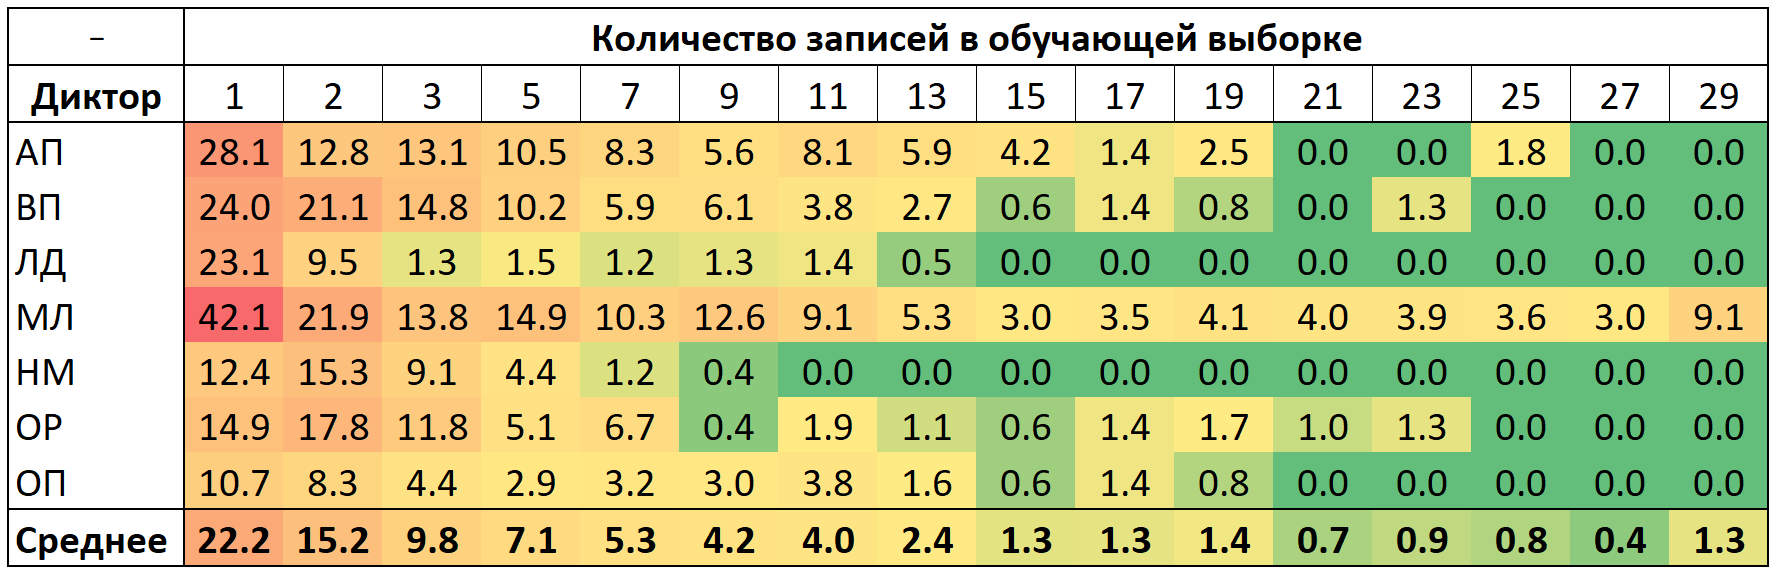
\includegraphics[width=1.0\textwidth]{cnn_phrases_self.png}
	\caption{Результаты распознавания фраз свёрточной нейронной сетью при обучении на других записях соответствующего диктора, в таблице указан процент неправильных распознаваний}
	\label{fig:cnn_phrases_self}
\end{figure}

Видно, что достаточно обучиться на 9 записях, чтобы ошибка стала ниже 5~\%, на 15 записях, чтобы стала ниже 2~\% и на 21 записи для 1~\% ошибок.

Аналогично распознаванию слов проводилось распознавание фраз при обучении нейронной сети на данных одного диктора в условиях без шума.
При распознавании слов из обучающей выборки в среднем получается 0.0~\% ошибок, а для распознавания слов из тестовой выборки --- 18.0~\% ошибок.
Подробные результаты приведены в таблице \ref{tab:cnn_phrases_1dictor}.

\begin{table}[h]
	\centering
	\caption{Результаты распознавания фраз свёрточной нейронной сетью на обучающем наборе из одного диктора в условиях без шума, в таблице указан процент неправильных распознаваний}
	\label{tab:cnn_phrases_1dictor}
	\begin{tabular}{| l | c | c | c | c | c | c | c |}
		\hline
		Набор & \multicolumn{7}{c|}{Диктор для распознавания} \\
		\hhline{~-------}
		обучения \phantom{0000} & \phantom{0} АП \phantom{0} & \phantom{0} ВП \phantom{0} & \phantom{0} ЛД \phantom{0} & \phantom{0} МЛ \phantom{0} & \phantom{0} НМ \phantom{0} & \phantom{0} ОР \phantom{0} & \phantom{0} ОП \phantom{0} \\
		\hline
		АП 		 &  0.0 & 31.2 & 61.2 & 20.3 & 36.4 & 43.6 & 13.9 \\
		ВП 		 & 21.5 &  0.0 & 12.1 & 21.5 &  3.0 &  9.4 &  9.7 \\
		ЛД 		 & 37.6 &  7.9 &  0.0 & 21.8 & 13.0 & 21.2 & 18.8 \\
		МЛ 		 & 10.0 & 10.3 & 13.3 &  0.0 &  5.5 & 15.5 &  2.1 \\
		НМ 		 & 30.0 &  6.4 & 11.2 & 22.1 &  0.0 & 18.2 &  7.3 \\
		ОР 		 & 41.2 &  9.4 & 18.2 & 24.8 &  9.4 &  0.0 & 10.3 \\
		ОП 		 & 16.1 & 10.3 & 23.0 & 11.2 &  9.7 & 17.9 &  0.0 \\
		\hline
	\end{tabular}
\end{table}

Далее было проведено распознавание фраз с помощью трёх дикторов.
При распознавании фраз из обучающей выборки в среднем получается 0.0~\% ошибок, а для распознавания слов из тестовой выборки --- 6.9~\% ошибок.
Подробные результаты приведены в таблице \ref{tab:cnn_phrases_3dictors}.

\begin{table}[h]
	\centering
	\caption{Результаты распознавания фраз свёрточной нейронной сетью на обучающем наборе из трёх дикторов в условиях без шума, в таблице указан процент неправильных распознаваний}
	\label{tab:cnn_phrases_3dictors}
	\begin{tabular}{| l | c | c | c | c | c | c | c |}
		\hline
		Набор & \multicolumn{7}{c|}{Диктор для распознавания} \\
		\hhline{~-------}
		обучения \phantom{0000} & \phantom{0} АП \phantom{0} & \phantom{0} ВП \phantom{0} & \phantom{0} ЛД \phantom{0} & \phantom{0} МЛ \phantom{0} & \phantom{0} НМ \phantom{0} & \phantom{0} ОР \phantom{0} & \phantom{0} ОП \phantom{0} \\
		\hline
		АП,ВП,ЛД &  0.0 &  0.0 &  0.0 &  5.2 &  1.5 & 12.4 &  2.7 \\
		ВП,ЛД,МЛ & 10.0 &  0.0 &  0.0 &  0.0 &  2.4 &  7.9 &  1.2 \\
		ЛД,МЛ,НМ & 12.7 &  5.8 &  0.0 &  0.0 &  0.0 &  8.8 &  3.0 \\
		МЛ,НМ,ОР & 13.6 &  5.8 &  5.5 &  0.0 &  0.0 &  0.0 &  1.5 \\
		НМ,ОР,ОП & 26.4 &  4.8 &  7.0 & 11.8 &  0.0 &  0.0 &  0.0 \\
		ОР,ОП,АП &  0.0 &  3.6 &  9.7 &  6.1 &  4.2 &  0.0 &  0.0 \\
		ОП,АП,ВП &  0.0 &  0.0 &  3.6 &  5.8 &  3.0 &  6.1 &  0.0 \\
		\hline
	\end{tabular}
\end{table}

Для распознавания несколькими дикторами были составлены несколько наборов данных для обучения.
Каждый набор состоит из записей фраз 6 различных дикторов.
Далее на нейронных сетях, обученных на приведённых наборах, производились распознавания на обучающей и тестовой выборках.
Как видно из таблицы \ref{tab:cnn_phrases_6dictors}, для случая фраз без шума средний результат лучше, чем при распознавании одним или тремя дикторами.

\begin{table}[h]
	\centering
	\caption{Результаты распознавания фраз свёрточной нейронной сетью на обучающем наборе из шести дикторов в условиях без шума, в таблице указан процент неправильных распознаваний}
	\label{tab:cnn_phrases_6dictors}
	\begin{tabular}{| l | c | c | c | c | c | c | c |}
		\hline
		Набор & \multicolumn{7}{c|}{Диктор для распознавания} \\
		\hhline{~-------}
		обучения & \phantom{0}АП\phantom{0} & \phantom{0}ВП\phantom{0} & \phantom{0}ЛД\phantom{0} & \phantom{0}МЛ\phantom{0} & \phantom{0}НМ\phantom{0} & \phantom{0}ОР\phantom{0} & \phantom{0}ОП\phantom{0} \\
		\hline
		АП,ВП,ЛД,МЛ,НМ,ОР	 &  0.0 &  0.0 &  0.0 &  0.0 &  0.0 &  0.0 &  1.5 \\
		ВП,ЛД,МЛ,НМ,ОР,ОП	 & 10.0 &  0.0 &  0.0 &  0.0 &  0.0 &  0.0 &  0.0 \\
		ЛД,МЛ,НМ,ОР,ОП,АП	 &  0.0 &  2.4 &  0.0 &  0.0 &  0.0 &  0.0 &  0.0 \\
		МЛ,НМ,ОР,ОП,АП,ВП	 &  0.0 &  0.0 &  3.3 &  0.0 &  0.0 &  0.0 &  0.0 \\
		НМ,ОР,ОП,АП,ВП,ЛД	 &  0.0 &  0.0 &  0.0 &  5.5 &  0.0 &  0.0 &  0.0 \\
		ОР,ОП,АП,ВП,ЛД,МЛ	 &  0.0 &  0.0 &  0.0 &  0.0 &  0.6 &  0.0 &  0.0 \\
		ОП,АП,ВП,ЛД,МЛ,НМ	 &  0.0 &  0.0 &  0.0 &  0.0 &  0.0 &  5.8 &  0.0 \\
		\hline
	\end{tabular}
\end{table}

При распознавании слов из обучающей выборки ошибок нет, а для распознавания слов из тестовой выборки в среднем получается 4.2~\% ошибок.

В таблице \ref{tab:cnn_phrases_without_noise_summary} приведены суммарные результаты распознавания фраз без шума при обучении на различном количестве дикторов.

\begin{table}[h]
	\centering
	\caption{Суммарные результаты распознавания при обучении на наборе из различного числа дикторов для случая фраз без шума}
	\label{tab:cnn_phrases_without_noise_summary}
	\begin{tabular}{| l | c | c | c | c | c | c |}
		\hline
		Количество дикторов \phantom{00} & \phantom{00} 1 \phantom{00} & \phantom{00} 2 \phantom{00} & \phantom{00} 3 \phantom{00} & \phantom{00} 4 \phantom{00} & \phantom{00} 5 \phantom{00} & \phantom{00} 6 \phantom{00} \\
		\hline
		Процент ошибок 		& 18.0 & 11.4 & 6.9 & 5.4 & 4.8 & 4.2 \\
		\hline
	\end{tabular}
\end{table}

Как и при распознавании слов, можно сделать вывод, что процент ошибок стабильно снижается при увеличении количества дикторов в обучающей базе из-за уменьшения дикторозависимости.

После этого производилось обучение и распознавание фраз в условиях шума кабины пилотов.
Шум моделировался аналогично моделированию для случая слов --- для каждой из фраз использовался уникальный шум, обеспечивающий одинаковое отношение сигнал/шум, как и в эксперименте по распознаванию отдельных слов в условиях шума.

В начале проводился эксперимент по распознаванию записей того же диктора, записи которого использовались в качестве обучающей выборки.
Результаты этих распознаваний приведены на рисунке \ref{fig:cnn_phrases_self_noise}.
По столбцам отложено количество записей для каждого слова, содержащихся в обучающей выборке, а в столбцах указан используемый уровень шума.
Приведённые результаты являются усреднёнными значениями по всем использованным дикторам.

\begin{figure}[h]
	\centering
	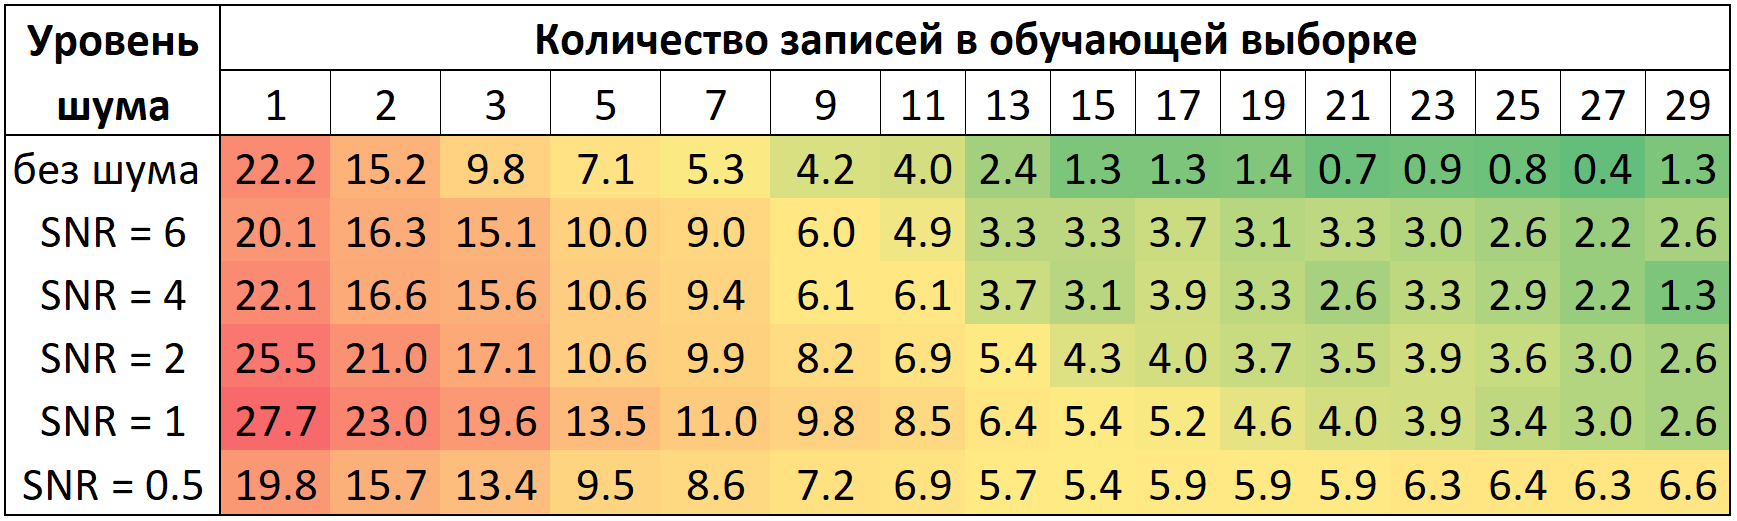
\includegraphics[width=1.0\textwidth]{cnn_phrases_self_noise.png}
	\caption{Усреднённые результаты распознавания фраз свёрточной нейронной сетью в условиях различных уровней шума при обучении на том же дикторе, в таблице указан процент неправильных распознаваний}
	\label{fig:cnn_phrases_self_noise}
\end{figure}

В данных результатах, аналогично результатам распознавания слов, видно плавное повышение процента ошибок при увеличении уровня шума, при этом по величине повышение оказывается не очень большим.
Например, при использовании 13 записей в обучающей выборке при отсутствии шума получается 2.4~\% ошибок, а при отношении сигнал/шум равном 1 получается 6.4~\% ошибок.
Аналогичные значения при обучении на 9 записях равны 4.2 и 9.8~\% соответственно.
Данные результаты показывают, к каким величинам ошибок нужно стремиться при распознавании фраз с шумом других дикторов для исключения эффекта дикторозависимости.

Далее отношение сигнал/шум принималось равным 4.
Также были эксперименты с наложением нескольких различных вариантов шумов на одни и те же записи.
Для начала было проведено обычное распознавание фраз одним диктором с наложением одного варианта шума.
В таблице \ref{tab:cnn_phrases_1dictor_1noise} представлено 2 варианта эксперимента.

\begin{table}[h]
	\centering
	\caption{Результаты распознавания фраз для случая записей с шумом при распознавании на обучающем наборе из одного диктора с 1 вариантом шума, в таблице указан процент неправильных распознаваний}
	\label{tab:cnn_phrases_1dictor_1noise}
	\begin{tabular}{| l | c | c | c | c | c | c | c |}
		\hline
		Набор & \multicolumn{7}{c|}{Диктор для распознавания} \\
		\hhline{~-------}
		обучения \phantom{0000} & \phantom{0} АП \phantom{0} & \phantom{0} ВП \phantom{0} & \phantom{0} ЛД \phantom{0} & \phantom{0} МЛ \phantom{0} & \phantom{0} НМ \phantom{0} & \phantom{0} ОР \phantom{0} & \phantom{0} ОП \phantom{0} \\
		\hline
		\multicolumn{8}{|c|}{обучение с шумом, распознавание без шума} \\
		\hline
		АП		 &  0.0 & 38.5 & 45.5 & 15.2 & 34.8 & 50.0 & 11.8 \\
		ВП		 & 40.3 &  0.6 & 16.7 & 31.2 & 15.8 & 21.2 & 17.3 \\
		ЛД		 & 47.0 & 19.4 &  0.0 & 24.5 & 15.8 & 22.4 & 24.5 \\
		МЛ		 & 20.0 & 17.0 & 22.1 &  0.6 & 19.7 & 15.8 &  1.2 \\
		НМ		 & 41.2 &  7.6 & 15.8 & 25.2 &  0.0 & 12.4 & 10.3 \\
		ОР		 & 48.2 & 14.2 & 23.0 & 36.4 & 17.3 &  0.0 & 18.8 \\
		ОП		 & 22.1 & 16.4 & 33.9 & 17.0 & 18.2 & 26.7 &  0.6 \\
		\hline
		\multicolumn{8}{|c|}{обучение с шумом, распознавание с шумом} \\
		\hline
		АП		 &  0.0 & 36.1 & 46.1 & 21.5 & 37.6 & 49.4 & 17.6 \\
		ВП		 & 33.6 &  0.0 & 12.1 & 24.2 & 10.9 & 20.9 & 11.5 \\
		ЛД		 & 44.8 & 14.8 &  0.0 & 26.1 & 14.8 & 33.9 & 19.1 \\
		МЛ		 & 12.7 & 18.5 & 17.9 &  0.0 & 12.1 & 20.3 &  3.6 \\
		НМ		 & 37.3 &  8.5 & 10.6 & 23.6 &  0.0 & 29.1 & 10.6 \\
		ОР		 & 47.3 & 13.3 & 20.6 & 33.9 & 15.2 &  0.0 & 17.0 \\
		ОП		 & 21.5 & 18.5 & 23.3 & 11.8 & 14.2 & 22.4 &  0.0 \\
		\hline
	\end{tabular}
\end{table}

В первом случае обучение проводилось на фразах с шумом, а распознавались фразы без шума.
Средняя ошибка при распознавании записей диктора, на которых проводилось обучение, равна 0.3~\%, а средняя ошибка для записей других дикторов --- 23.6~\%.
Во втором случае и обучение, и распознавание проводилось на записях с шумом.
На записях, на которых проводилось обучение, ошибок не было, а средняя ошибка для записей других дикторов равна 22.4~\%.
Из этих результатов видно, что для обоих вариантов распознавания ошибка получается выше, чем при использовании записей без шума.
Более того, аналогично распознаванию слов распознавание записей с шумом показало меньшую ошибку, чем распознавание записей без шума.
В дальнейшем будет использоваться только распознавание записей с шумом.

Далее был проведён аналогичный эксперимент, но с тем отличием, что для обучения использовались записи с 5 и 10 наложенными различными вариантами шума.
Для первого эксперимента с 5 вариантами шума средняя ошибка при распознавании записей диктора, на которых проводилось обучение, равна 0.0~\%, а средняя ошибка для записей других дикторов --- 21.1~\%.
Для второго эксперимента с 10 вариантами шума на записях, на которых проводилось обучение, ошибок не было, а средняя ошибка для записей других дикторов равна 20.8~\%.
Как видно из приведённых результатов, использование нескольких вариантов шумов заметно улучшает качество распознавания по сравнению с 1 вариантом шума.
Результаты данных экспериментов приведены в таблице \ref{tab:cnn_phrases_1dictor_noises}.

\begin{table}[h]
	\centering
	\caption{Результаты распознавания фраз для случая записей с шумом при распознавании на обучающем наборе из одного диктора с 5 и 10 вариантами шума, в таблице указан процент неправильных распознаваний}
	\label{tab:cnn_phrases_1dictor_noises}
	\begin{tabular}{| l | c | c | c | c | c | c | c |}
		\hline
		Набор & \multicolumn{7}{c|}{Диктор для распознавания} \\
		\hhline{~-------}
		обучения \phantom{0000} & \phantom{0} АП \phantom{0} & \phantom{0} ВП \phantom{0} & \phantom{0} ЛД \phantom{0} & \phantom{0} МЛ \phantom{0} & \phantom{0} НМ \phantom{0} & \phantom{0} ОР \phantom{0} & \phantom{0} ОП \phantom{0} \\
		\hline
		\multicolumn{8}{|c|}{5 вариантов шума} \\
		\hline
		АП 		 &  0.0 & 35.5 & 43.9 & 17.9 & 40.0 & 42.7 & 15.8 \\
		ВП 		 & 33.0 &  0.0 &  9.4 & 23.3 & 10.9 & 22.7 & 13.0 \\
		ЛД		 & 42.1 & 10.3 &  0.0 & 23.3 & 12.1 & 28.8 & 18.8 \\
		МЛ		 & 11.5 & 14.5 & 13.6 &  0.0 & 13.3 & 17.6 &  3.0 \\
		НМ		 & 42.7 & 10.9 & 13.0 & 23.3 &  0.0 & 27.3 & 10.9 \\
		ОР		 & 47.0 & 11.5 & 19.4 & 33.0 & 11.2 &  0.0 & 13.0 \\
		ОП		 & 23.0 & 14.2 & 21.2 & 12.4 & 12.1 & 23.6 &  0.0 \\
		\hline
		\multicolumn{8}{|c|}{10 вариантов шума} \\
		\hline
		АП		 &  0.0 & 37.0 & 45.8 & 18.5 & 38.5 & 44.5 & 15.2 \\
		ВП		 & 35.2 &  0.0 & 16.7 & 23.9 & 10.9 & 19.7 & 10.9 \\
		ЛД		 & 40.0 & 10.6 &  0.0 & 20.9 & 10.9 & 28.8 & 15.5 \\
		МЛ		 & 11.8 & 13.0 & 12.7 &  0.0 &  9.7 & 16.7 &  2.4 \\
		НМ		 & 44.8 & 10.9 & 10.9 & 23.3 &  0.0 & 27.9 & 10.9 \\
		ОР		 & 48.2 & 15.8 & 22.4 & 29.4 & 14.2 &  0.0 & 12.4 \\
		ОП		 & 23.6 & 13.6 & 19.7 &  9.7 & 10.6 & 17.0 &  0.0 \\
		\hline
	\end{tabular}
\end{table}

После этого было проведено обучение нейронной сети на 3 дикторах в условиях шума и последующее распознавания записей.
Первый эксперимент предполагает использование одного варианта шума при обучении, а второй эксперимент --- 5 вариантов шума.
В обоих случаях средняя величина ошибки при распознавании записей диктора, на которых проводилось обучение, равна 0.0~\%.
Для случая распознавания записей других дикторов ошибка равна 11.5~\% для первого эксперимента и 10.4~\% для второго.
Подробные результаты экспериментов приведены в таблице \ref{tab:cnn_phrases_3dictors_noises}.

\begin{table}[h]
	\centering
	\caption{Результаты распознавания фраз для случая записей с шумом при распознавании на обучающем наборе из трёх дикторов с 1 и 5 вариантами шума, в таблице указан процент неправильных распознаваний}
	\label{tab:cnn_phrases_3dictors_noises}
	\begin{tabular}{| l | c | c | c | c | c | c | c |}
		\hline
		Набор & \multicolumn{7}{c|}{Диктор для распознавания} \\
		\hhline{~-------}
		обучения \phantom{0000} & \phantom{0} АП \phantom{0} & \phantom{0} ВП \phantom{0} & \phantom{0} ЛД \phantom{0} & \phantom{0} МЛ \phantom{0} & \phantom{0} НМ \phantom{0} & \phantom{0} ОР \phantom{0} & \phantom{0} ОП \phantom{0} \\
		\hline
		\multicolumn{8}{|c|}{1 вариант шума} \\
		\hline
		АП,ВП,ЛД &  0.0 & 0.0 &  0.0 &  8.2 &  6.4 & 20.3 & 6.4 \\
		ВП,ЛД,МЛ & 14.5 & 0.0 &  0.0 &  0.0 &  6.1 & 17.3 & 3.9 \\
		ЛД,МЛ,НМ & 16.4 & 7.0 &  0.0 &  0.0 &  0.0 & 17.9 & 1.8 \\
		МЛ,НМ,ОР & 17.6 & 7.0 &  7.9 &  0.0 &  0.0 &  0.0 & 1.5 \\
		НМ,ОР,ОП & 28.2 & 9.7 & 11.2 & 15.8 &  0.0 &  0.0 & 0.0 \\
		ОР,ОП,АП &  0.0 & 9.1 & 20.6 &  7.0 & 12.4 &  0.0 & 0.0 \\
		ОП,АП,ВП &  0.0 & 0.0 & 12.7 &  8.2 &  9.1 & 18.5 & 0.0 \\
		\hline
		\multicolumn{8}{|c|}{5 вариантов шума} \\
		\hline
		АП,ВП,ЛД &  0.0 & 0.0 &  0.0 &  8.2 &  8.2 & 17.3 & 4.5 \\
		ВП,ЛД,МЛ & 13.6 & 0.0 &  0.0 &  0.0 &  7.6 & 14.2 & 0.9 \\
		ЛД,МЛ,НМ & 15.5 & 5.8 &  0.0 &  0.0 &  0.0 & 18.2 & 2.4 \\
		МЛ,НМ,ОР & 17.9 & 8.2 &  5.8 &  0.0 &  0.0 &  0.0 & 1.2 \\
		НМ,ОР,ОП & 27.6 & 6.4 &  9.1 & 13.6 &  0.0 &  0.0 & 0.0 \\
		ОР,ОП,АП &  0.0 & 7.3 & 15.8 &  7.9 & 11.2 &  0.0 & 0.0 \\
		ОП,АП,ВП &  0.0 & 0.0 & 12.1 &  6.7 & 10.6 & 13.3 & 0.0 \\
		\hline
	\end{tabular}
\end{table}

Здесь также видно улучшение при увеличении вариантов шума в обучающей выборке.

Результаты эксперимента на фразах с наложенным шумом при обучении на 7 дикторах приведены в таблице \ref{tab:cnn_phrases_7dictors_noises}.

\begin{table}[h]
	\centering
	\caption{Результаты распознавания фраз для случая записей с шумом при распознавании на обучающем наборе из семи дикторов с 1 и 2 вариантами шума, в таблице указан процент неправильных распознаваний}
	\label{tab:cnn_phrases_7dictors_noises}
	\begin{tabular}{| l | c | c | c | c | c | c | c |}
		\hline
		Набор & \multicolumn{7}{c|}{Диктор для распознавания} \\
		\hhline{~-------}
		обучения & \phantom{0}АП\phantom{0} & \phantom{0}ВП\phantom{0} & \phantom{0}ЛД\phantom{0} & \phantom{0}МЛ\phantom{0} & \phantom{0}НМ\phantom{0} & \phantom{0}ОР\phantom{0} & \phantom{0}ОП\phantom{0} \\
		\hline
		\multicolumn{8}{|c|}{1 вариант шума} \\
		\hline
		АП,ВП,ЛД,МЛ,НМ,ОР &  0.0 & 0.0 & 0.0 & 0.0 & 0.0 &  0.0 & 2.4 \\
		ВП,ЛД,МЛ,НМ,ОР,ОП & 16.7 & 0.0 & 0.0 & 0.0 & 0.0 &  0.0 & 0.0 \\
		ЛД,МЛ,НМ,ОР,ОП,АП &  0.0 & 5.5 & 0.0 & 0.0 & 0.0 &  0.0 & 0.0 \\
		МЛ,НМ,ОР,ОП,АП,ВП &  0.0 & 0.0 & 5.2 & 0.0 & 0.0 &  0.0 & 0.0 \\
		НМ,ОР,ОП,АП,ВП,ЛД &  0.0 & 0.0 & 0.0 & 7.9 & 0.0 &  0.0 & 0.0 \\
		ОР,ОП,АП,ВП,ЛД,МЛ &  0.0 & 0.0 & 0.0 & 0.0 & 5.5 &  0.0 & 0.0 \\
		ОП,АП,ВП,ЛД,МЛ,НМ &  0.0 & 0.0 & 0.0 & 0.0 & 0.0 & 15.8 & 0.0 \\
		\hline
		\multicolumn{8}{|c|}{2 варианта шума} \\
		\hline
		АП,ВП,ЛД,МЛ,НМ,ОР &  0.0 & 0.0 & 0.0 & 0.0 & 0.0 &  0.0 & 1.2 \\
		ВП,ЛД,МЛ,НМ,ОР,ОП & 13.9 & 0.0 & 0.0 & 0.0 & 0.0 &  0.0 & 0.0 \\
		ЛД,МЛ,НМ,ОР,ОП,АП &  0.0 & 6.1 & 0.0 & 0.0 & 0.0 &  0.0 & 0.0 \\
		МЛ,НМ,ОР,ОП,АП,ВП &  0.0 & 0.0 & 6.1 & 0.0 & 0.0 &  0.0 & 0.0 \\
		НМ,ОР,ОП,АП,ВП,ЛД &  0.0 & 0.0 & 0.0 & 7.0 & 0.0 &  0.0 & 0.0 \\
		ОР,ОП,АП,ВП,ЛД,МЛ &  0.0 & 0.0 & 0.0 & 0.0 & 3.6 &  0.0 & 0.0 \\
		ОП,АП,ВП,ЛД,МЛ,НМ &  0.0 & 0.0 & 0.0 & 0.0 & 0.0 & 10.9 & 0.0 \\
		\hline
	\end{tabular}
\end{table}

В данном эксперименте при обучении использовались один и два варианта шума.
Большее количество шумов не удалось использовать из-за ограничений вычислительной мощности компьютера.
Для обоих вариантов обучения, при распознавании фраз из обучающей выборки ошибок нет.
При использовании одного варианта шума, для распознавания фраз из тестовой выборки получается в среднем 8.4~\% ошибок, а при использовании двух вариантов шума --- 7.0~\% ошибок.

В таблице \ref{tab:cnn_phrases_with_noise_summary} приведены итоговые результаты распознавания фраз в условиях шума при обучении на различном числе дикторов и различном количестве наложенных шумов.

\begin{table}[h]
	\centering
	\caption{Суммарные результаты распознавания по <<своему>> и <<чужому>> диктору при обучении на различном числе дикторов для случаев записей фраз без шума и с шумом, в таблице указан процент неправильных распознаваний}
	\label{tab:cnn_phrases_with_noise_summary}
	\begin{tabular}{| l | c | c | c | c |}
		\hline
		Число				& \phantom{0}Наличие\phantom{0} & \phantom{0} Число \phantom{0} 	& \multicolumn{2}{c|}{Процент ошибок}	\\
		\hhline{~~~--}
		дикторов			& шума  			& шумов 	& обучающая выборка & тестовая выборка	\\
		\hline
		\multirow{4}{*}{1 диктор}	& без шума					& 1				& 0.3 		& 23.6 		\\
		\hhline{~----}
									& \multirow{3}{*}{с шумом}	& 1				& 0.0 		& 22.4  	\\
		\hhline{~~---}
									&							& 5				& 0.0 		& 21.1  	\\
		\hhline{~~---}
									&    						& 10			& 0.0 		& 20.8  	\\
		\hline
		\multirow{2}{*}{3 диктора}	& \multirow{2}{*}{с шумом}	& 1				& 0.0 		& 11.5  	\\
		\hhline{~~---}
									&    						& 5				& 0.0 		& 10.4  	\\
		\hline
		\multirow{2}{*}{6 дикторов}	& \multirow{2}{*}{с шумом}	& 1				& 0.0 		& 8.4  		\\
		\hhline{~~---}
									&    						& 2				& 0.0 		& 7.0  		\\
		\hline
	\end{tabular}
\end{table}

Здесь получается вывод, полностью аналогичный выводу, полученному в экспериментах распознавания слов в условиях шума: процент ошибок стабильно снижается при увеличении количества дикторов в обучающей базе и увеличение числа накладываемых шумов приводит к уменьшению числа ошибок, но уменьшение меньше, чем при увеличении количества дикторов.

В целом, результаты распознавания фраз очень похожи на результаты распознавания слов, как в условиях без шума, так и в условиях с шумом.
Единственное отличие --- это заметно большее количество ошибок.
Это можно объяснить тем, что при произношении фраз большую роль играет длительность паузы между словами, в то время как при распознавании слов такой проблемы не возникает.
Но, в любом случае, свёрточные нейронные сети показали лучшие результаты для задачи распознавания фраз.

\clearpage

%\newpage
%============================================================================================================================

\section{Улучшение качества распознавания отдельных фраз при дополнительном обучении} \label{sect4_6}

В конце был проведён эксперимент по расширению обучающей выборки и исследованию изменения качества распознавания.
Эксперимент заключался в следующем.
Предположим, что у нас есть обучающая выборка из записей одного или нескольких дикторов.
Нейронная сеть обучается на данной выборке.
После этого с помощью нейронной сети распознаются записи другого диктора, не входящего в обучающую выборку.
Таким образом, реализуется вариант распознавания по <<чужому>> диктору.

После этого было проверено изменение качества распознавания команд при обучении по записям чужого диктора с добавлением небольшого числа записей своего диктора, то есть того, чьи записи будут потом распознаваться.
При этом, несмотря на то, что записи из обучающей выборки и записи для распознавания будут принадлежать одному диктору, это будут разные реализации команд, то есть добавленные к обучающей выборке записи исключаются из тестовой выборки.
В обучающую выборку добавлялось 1, 2, 3, 5, 10 и 15 записей своего диктора.
Таким образом, можно учесть некоторые индивидуальные особенности распознаваемого диктора при добавлении лишь небольшого числа записей, что достаточно несложно реализуется на практике.

В таблице \ref{tab:cnn_phrases_addition} приведены результаты распознавания в эксперименте для различных наборов параметров.
В строках указано количество использованных в обучающей выборке <<чужих>> дикторов.
По столбцам отложено количество записей каждого слова <<своего>> диктора, добавленных в обучающую выборку.

\begin{table}[h]
	\centering
	\caption{Процент ошибок распознавания фраз при добавлении различного количества записей к обучающей выборке, состоящей из записей одного или нескольких дикторов}
	\label{tab:cnn_phrases_addition}
	\begin{tabular}{| l | c | c | c | c | c | c | c |}
		\hline
		Число & \multicolumn{7}{c|}{Число добавленных записей} \\
		\hhline{~-------}
		дикторов \phantom{000} & \phantom{00} 0 \phantom{00} & \phantom{00} 1 \phantom{00} & \phantom{00} 2 \phantom{00} & \phantom{00} 3 \phantom{00} & \phantom{00} 5 \phantom{00} & \phantom{00} 10 \phantom{00} & \phantom{00} 15 \phantom{00} \\
		\hline
		1 		 & 18.0 & 8.8 & 7.2 & 6.4 & 5.2 & 3.7 & 1.9 \\
		2 		 & 11.4 & 7.1 & 6.1 & 5.2 & 4.8 & 3.6 & 1.6 \\
		3 		 &  6.9 & 5.2 & 4.8 & 4.3 & 3.8 & 3.1 & 1.2 \\
		4 		 &  5.4 & 4.6 & 3.7 & 3.7 & 3.2 & 2.7 & 1.1 \\
		5 		 &  4.8 & 4.3 & 4.1 & 3.9 & 3.5 & 2.7 & 1.2 \\
		6 		 &  4.2 & 3.9 & 3.8 & 3.7 & 3.2 & 2.9 & 1.2 \\
		\hline
	\end{tabular}
\end{table}

Как видно из результатов, при добавлении всего по одной реализации каждой из речевых команд <<своего>> диктора в обучающую выборку ошибка распознавания уменьшается более чем в 2 раза с 18.6 до 8.8~\%.
Дальнейшее добавление записей снижает ошибку, но величина снижения уже не такая большая.
Также, эффект от добавленных записей тем больше, чем меньше дикторов использовано в обучающей выборке.
Это объясняется тем, что при маленьком числе дикторов в обучающей выборке высока степень переобучения для конкретного диктора, поэтому добавление записей другого диктора хорошо снижает степень такого переобучения.
Для обучающих выборок из нескольких дикторов переобучение меньше, поэтому меньше и улучшение.
При добавлении нескольких реализаций слов процент ошибок продолжает снижаться, но меньшими темпами.
Практический результат данного эксперимента состоит в том, что добавление небольшого числа записей к большой обучающей выборке заметно влияет на точность распознавания.

%\newpage
%============================================================================================================================

\section{Выводы по разработке алгоритмов на основе свёрточных нейронных сетей} \label{sect4_7}

В данном разделе описаны предложенные алгоритмы распознавания речевых команд на основе свёрточных нейронных сетей.
В начале описана используемая среда разработки и применённая параметризация обучающей выборки и распознаваемых речевых записей.
После этого проведён анализ работоспособности традиционных нейронных сетей типа одно- и двухслойных персептронов.
Средняя полученная доля неправильно распознанных слов на тестовой выборке получилась высокой и составила 20--25~\%.

Далее была предложена архитектура свёрточной нейронной сети и проведён подбор параметров данной сети.
Затем для нескольких поставленных задач производилось обучение и проверка результатов работы алгоритма.
Первой задачей было распознавание записей <<своего>> диктора.
Результаты показали, что можно добиться ошибки распознавания в 2~\% при использовании 7 записей каждого слова в обучающей выборке и ошибки в 0.5~\% для 20 записей.

Вторая задача заключалась в обучении на записях одного или нескольких дикторов и распознавании записей <<чужого>> диктора.
Здесь удалось получить долю ошибок равную 5.9~\% для обучающей выборки из одного диктора, 1.7~\% для выборки из 3 дикторов и 0.6~\% для 7 дикторов.
Последний результат является очень хорошим, так как результат распознавания <<чужого>> диктора вплотную приближается к результату распознавания по <<своему>> диктору.

Третья задача подразумевала проверку работоспособности свёрточных нейронных сетей при обучении и распознавании записей с шумом.
Для этого уникальные части шума кабины пилота добавлялись ко всем записям.
При распознавании записей <<своего>> диктора количество ошибок увеличилось примерно в 2 раза при использовании отношения сигнал/шум равного 1.
Также было показано стабильное, но не очень большое по величине повышение числа ошибок при увеличении уровня шума.
При распознавании записей <<чужого>> диктора были получены ошибки равные 9.7~\% при обучении на записях одного диктора с одним добавленным шумом, а если добавлялось 7 различных вариантов шума в обучающую выборку, то ошибка снижалась до 8.2~\%.
Для 3 дикторов процент ошибок был 2.8~\% для одно варианта шума и 2.5~\% для 3 вариантов.
Для 7 дикторов эти значения были соответственно 1.2 и 1.1~\%, что является крайне низким значением при распознавании в условиях шума.

После этого были проведены аналогичные эксперименты для речевых команд в форме фраз.
Для распознавания по <<своему>> диктору было получено около 1~\% ошибок при размере обучающей выборки в 20 записей каждого слова.
Распознавание по <<чужому>> диктору показало 18~\% ошибок при обучении по записям одного диктора, 6.9~\% ошибок при 3 дикторах и 4.2~\% для 6 дикторов.
При распознавании записей <<своего>> диктора в условиях шума получены результаты аналогичные случаю распознавания слов.
При распознавании записей <<чужих>> дикторов с шумом для 1 диктора получилось от 20.8 до 23.6~\% ошибок и от 7.0 до 8.4~\% ошибок для обучающей выборки из записей 6 дикторов.

В конце был рассмотрен способ улучшения качества распознавания за счёт добавлению к обучающей выборке небольшого количества записей <<своего>> диктора.
Получилось, что при добавлении всего 1 реализации каждого слова в обучающую выборку, состоящую из записей одного диктора, доля ошибок снижалась с 18 до 8.8~\%, а при добавлении 3 записей до 6.4~\%.
Для обучающей выборки из 3 дикторов при добавлении одной записи было зафиксировано снижение числа неправильных распознаваний с 6.9 до 5.2~\%, а при добавлении 3 записей до 4.3~\%.
По результатам видно, что добавление всего лишь 1 записи каждого слова <<своего>> диктора приводит к сильному снижению процента ошибок распознавания, особенно при обучении на выборках с записями малого количества дикторов.

%\newpage
%============================================================================================================================

\clearpage